% das Papierformat zuerst
\documentclass[a4paper, 11pt]{article}
%more colors
\usepackage[dvipsnames]{xcolor}
% deutsche Silbentrennung
\usepackage[ngerman]{babel}
% wegen deutschen Umlauten
\usepackage[utf8]{inputenc}
% andere pdfs einbinden
\usepackage{pdfpages}
% um bilder einzubinden
\usepackage{graphicx}
% fuer source code listings
\usepackage{listings}
% seitenränder
\usepackage[left=3cm,right=3cm,top=2cm,bottom=2cm]{geometry}
% um hyperlinks einfügen zu können
\usepackage{hyperref}
% um weitere Symbole zu nutzen
\usepackage{amssymb}
% um weitere Operatoren zu nutzen
\usepackage{amsmath}
%Aufzaehlung
\usepackage{paralist}
%Beachtet, ob ein Leerzeichen syntaktisch passt oder nicht
\usepackage{xspace}
% um hyperlinks einfügen zu können
\usepackage{hyperref}
%um Kopf- und Fußzeile zu bearbeiten
\usepackage{fancyhdr}
%um Literaturverzeichnis auch im Inhaltsverzeichnis anzuzeigen
\usepackage{tocbibind}
%um Silbentrennungen angeben zu können, welche nicht unterstützt werden
\RequirePackage[ngerman=ngerman-x-latest]{hyphsubst}
%um Tabellen zu begrenzen, damit sie nicht in den Rand hineinragen
\usepackage{tabularx}
%um die landscape Umgebung zu nutzen (Querformat)
\usepackage{pdflscape}
%Stellt eine caption-Anweisung mit direkter Angabe des Gleitumgebungstyps bereit.
\usepackage{capt-of}
\usepackage{caption}
%ermöglicht die Option H für table
\usepackage{float}

%ermöglicht Anführungsstriche unten und oben
\newcommand{\su}{\glqq} %unten
\newcommand{\so}{\grqq\xspace} %oben mit anschließendem Leerzeichen
\newcommand{\soo}{\grqq} %nur oben

%ermöglicht eckige Klammern
\newcommand{\eka}{$<$} %<
\newcommand{\ekz}{$>$\xspace} %> mit anschließendem Leerzeichen

%Versionsnummer
\newcommand{\version}{0.7}

% Tabellenabschnitt linksbündig
\newcommand{\ltab}{\raggedright\arraybackslash}
% Tabellenabschnitt zentriert
\newcommand{\ctab}{\centering\arraybackslash}
% Tabellenabschnitt rechtsbündig
\newcommand{\rtab}{\raggedleft\arraybackslash}

%Einstellungen für Fuß- und Kopfzeile
\pagestyle{fancy}
\fancyhf{}
\fancyhead[L]{\footnotesize M. Lüdemann $\cdot$ M. Butkereit $\cdot$ W. Schumacher $\cdot$ A. Melkonyan $\cdot$ M. Colbow $\cdot$ M. Cakir\\ Requirements and Design Documentation $\cdot$ ESEP WS2016(v\version) $\cdot$ HAW Hamburg}
%\fancyhead[C]{\footnotesize}
\fancyhead[R]{\footnotesize \today}
%\renewcommand{\headrulewidth}{0.0pt}
\fancyfoot[C]{\thepage}

%Stil des Literaturverzeichnisses bestimmen
\bibliographystyle{unsrt}

\begin{document}

% Den Titel festlegen
\title
{
    Requirements and Design Documentation\\
    \bigskip
    (RDD)\\
    \medskip
    {\normalsize Version \version}\\
    \bigskip
    ESEP - Praktikum - Wintersemester 2016/2017
}

% Autor/en
\author
{
\begin{tabular}{llll}
    Lüdemann&Mona&2212744&mona.luedemann1@haw-hamburg.de\\
    Butkereit&Marvin&2247550&marvin.butkereit@haw-hamburg.de\\
    Schumacher&Wilhelm&2245216&wilhelm.schumacher@haw-hamburg.de\\
    Melkonyan&Anushavan&2243668&anushavan.melkonyan@haw-hamburg.de\\
    Colbow&Marco&2177095&marco.colbow@haw-hamburg.de\\
    Cakir&Mehmet&2195657&mehmet.cakir@haw-hamburg.de
\end{tabular}
}

% Erstelle die Titelseite
\maketitle

\noindent {\large Änderungshistorie:}
\begin{table}[h]
    \begin{tabularx}{\textwidth}{|c|c|c|X|}
    \hline
    \textbf{Version} & \textbf{Author} & \textbf{Datum} & \centering \arraybackslash \textbf{Anmerkungen/Änderungen}\\
    \hline
    0.1&Mehmet Cakir&2016-10-18&Kapitel 1-4 und Testkonzept\\
    \hline
    0.2&Mehmet Cakir&2016-10-26&Korrekturen an Formulierung, Visualisierungen noch nicht festgelegt.\\
    \hline
    0.3&Mehmet Cakir&2016-11-03&Testtabellen umformatiert. Tests zu Grundfunktionen, HAL\_UML, Systemgrenzen, Systemarchitektur und Visualisierungsentscheidung sowie entsprechend kurzen Text hinzugefügt.\\
    \hline
    0.4&Mehmet Cakir&2016-11-16&Neugliederung der Kapitel 4 und 7, Systemkontexte zusammengeführt, verwendete Werkzeuge ergänzt, Zeitmessung und FSM/HSM eingepflegt, Abbildung 6 zur Zeiterfassung aktualisiert, diverse Umformulierungen.\\
    \hline
    0.5&Mehmet Cakir&2016-11-17&Aktualisiertes UML-Klassendiagramm der HAL und Tests der Sensorik eingefügt.\\
    \hline
    0.6&Mehmet Cakir&2017-01-09&Einleitender Text, angepasster Terminplan, Tests und Dokumentation zur seriellen Schnittstelle, Implementierung(ISR, Threads und Dispatcher), Lessons Learned, Anregung zum Praktikum, Korrekturen an Ausdruck/Formulierung.\\
    \hline
    \end{tabularx}
\label{changes}
\end{table}

\newpage

\begin{table}[H]
    \begin{tabularx}{\textwidth}{|c|c|c|X|}
    \hline
    \textbf{Version} & \textbf{Author} & \textbf{Datum} & \centering \arraybackslash \textbf{Anmerkungen/Änderungen}\\
    \hline
    0.7&Mehmet Cakir&2017-01-09&Timer in Design umformuliert. Screenshots zu ISR, Threads und Dispatcher geändert. Zwei Unterkapitel aus Testen entfernt. Einleitung umformuliert. Verweis zu Milestones in Teamorganisation und Prozess geändert. Testkonzept für die Abnahme aktualisiert. SW-Architektur/Komponentendiagramm aktualisiert. Testszenarien hinzugefügt.\\
    \hline
    \end{tabularx}
\label{changes}
\end{table}

\newpage

\tableofcontents

\newpage

\section{Einleitung}
Diese Dokumentation beschreibt für dieses Projekt im Rahmen des ESE Praktika im Wintersemester 2016/2017 sämtliche Beschlüsse, Schritte und Maßnahmen die während des Projekt- bzw. Entwicklungszeitraums getroffen wurden. Das Projekt umfasst die Implementierung von Software zur Ansteuerung von drei baugleichen Förderbändern und die Kommunikation dieser untereinander des Unternehmens Festo, womit eine Werkstück-Sortieranlage realisiert werden soll. Über einen eigenen GEME-Rechner erfolgt die Ansteuerung pro Förderband. Zur Kommunikation der Förderbänder untereinander werden die GEME-Rechner über serielle Schnittstellen gekoppelt.

\section{Teamorganisation}
Grundsätzlich kann jedes Teammitglied eine Aufgabe seiner Wahl übernehmen. Bei jedem Meeting werden die Aufgaben verteilt, worüber im folgenden Meeting über den Fortschritt diskutiert wird. Falls ein Mitglied seine Aufgabe fertiggestellt hat, übernimmt er eine Neue. Bei Nichteinhaltung des Zeitplans werden entsprechend der Zeitpuffer andere Aufgaben zurückgestellt. Die Aufgaben richten sich nach den festgelegten Milestones im zum Projekt angefertigten Gantt Diagramm. Für die Projektleitung und die Pflege des RDD-Dokuments wurde jeweils eine Person bestimmt, welche im Unterkapitel \ref{vantw} eingesehen werden kann.

\subsection{Verantwortlichkeiten}\label{vantw}
\begin{table}[h]
\centering
    \begin{tabularx}{\textwidth}{|l|l|X|}
    \hline
    \textbf{Aufgabe}&\textbf{Zuständige/r}&\textbf{Bemerkung}\\
    \hline
    Projektleitung&Mona&Die Projektleitung überwacht den Projektfortschritt und benachrichtigt insbesondere bei Nichteinhalten des Zeitplans alle Teammitglieder. Außerdem hat die Projektleitung bei Unstimmigkeiten immer das letzte Wort. \\
    \hline
    RDD-Pflege&Mehmet&Der Zuständige ist für die Gestaltung und für die Vollständigkeit des RDDs verantwortlich. Er kann andere Gruppenmitglieder dazu auffordern Inhalte für das Dokument zu erarbeiten und ihm bereit zu stellen. \\
    \hline 
    Protkollführung&Alle Teammitglieder&Die Protokollführung wird reihum von Gruppenmitgliedern übernommen. Dabei wird folgende Reihenfolge eingehalten: $Mona\rightarrow Marvin\rightarrow Marco \rightarrow Wilhelm\rightarrow Mehmet\rightarrow Anushavan$ \\
    \hline
    \end{tabularx}
\caption{Zuteilung von Verantwortlichkeiten}
\label{labelname}
\end{table}

\subsection{Absprachen}
Zur Kommunikation außerhalb der Praktikumstermine werden die Messengerdienste Slack und WhatsApp verwendet. Unstimmigkeiten, Fragen und Inkenntnissetzungen können somit interaktiv geklärt bzw. mitgeteilt werden. Es wird erwartet, dass jedes Teammitglied in einem Zeitfenster von 24 Stunden auf eine Nachricht entsprechend mit einer Nachricht antwortet. In folgender Abbildung \ref{meets} werden die Termine der Meetings dargestellt:
\begin{figure}[h]
\centering 
    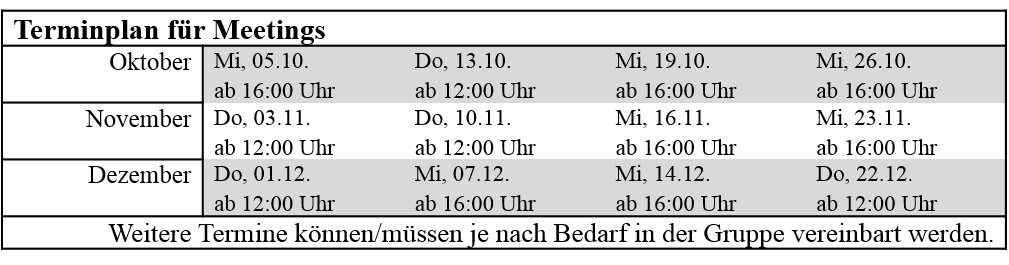
\includegraphics[scale=0.85]{images/Terminplan_Meetings.png}
    \caption{Terminplan der Meetings}
    \label{meets}
\end{figure}

\newpage

\subsection{Repository-Konzept}
Das Projekt wird mit dem Versionskontrollsystem Git verwaltet. Zentral wurde ein Repository auf GitHub angelegt. Erreichbar ist das Repository unter \url{https://github.com/mbutkereit/conveyor}. Änderungen werden lokal auf einem Branch vorgenommen, jedoch nicht auf dem Master. Sind die Änderungen erfolgreich abgeschlossen, kann der Master mit dem lokalen Branch zusammengeführt werden. Bevor ein push durchgeführt wird, muss gepullt werden. Nachdem ggf. Mergekonflikte gelöst wurden, kann vom Masterbranch aus auf das Repository gepusht werden.

\section{Projektmanagement}
Für die Gewährleistung einer guten Teamarbeit, werden in den folgenden Kapiteln erklärt wie die Teammitglieder mit ihren Aufgaben umgehen bzw. wann eine gegenseitige Benachrichtigung über ihren Fortschritt spätestens stattfinden sollte.

\subsection{Prozess}
Das Projekt wird auf Grundlage der festgelegten Milestones im zum Projekt angefertigten Gantt Diagramm umgesetzt. Für jede Implementierung ist zuvor ein geeignetes, sowie selbsterklärendes bzw. verständliches, aber auch möglichst vollständiges Diagramm anzufertigen. Die Visualisierung sollte vor der Implementierung allen anderen Teammitgliedern vorgestellt werden, um mögliche Verbesserungen einzuholen und ggf. Konflikte früh zu erkennen, sowie sie zu lösen. In der Tabelle \ref{visuals} sind für die jeweiligen Spezifikationen die festgelegte Modellierung aufgelistet.

\begin{table}[h]
\centering
    \begin{tabularx}{\textwidth}{|l|X|}
    \hline
    \textbf{Spezifikation}&\textbf{Modellierung}\\
    \hline
    Klassen&UML Diagramm\\
    \hline
    Verhalten bzw. logische Abläufe&Zustandsautomat\\
    \hline
    Systemarchitektur&Komponentendiagramm\\
    \hline
    \end{tabularx}
\caption{Festgelegte Modellierung zur jeweiligen Spezifikation}
\label{visuals}
\end{table}

\subsection{PSP/Zeitplan/Tracking}
Zu jedem Praktikumstermin wird erwartet, dass die verteilten Aufgaben bzw. Milestones erfüllt werden. Um dies zu gewährleisten, muss jedes Teammitglied bei Schwierigkeiten die Projektleitung darüber sofort in Kenntnis setzen, damit frühzeitig ausgeholfen werden kann. Dazu wurden Arbeitspakete definiert und als Milestones in einem Gantt-Diagramm festgehalten.

\subsection{Qualitätssicherung}
Hinsichtlich der Qualitätssicherung, werden die vier Punkte Team, Modellierung, Code und Förderband herangezogen.
\medskip
\begin{compactenum}[1.]
    \item \textbf{Team:} Jedes Teammitglied sollte über seine eigenen Fähigkeiten im Klaren sein und möglichst nur Aufgaben übernehmen, wofür es sich am besten geeignet fühlt. Darüber hinaus muss jedes Teammitglied bei Möglichkeit stets seine Unterstützung anbieten. Bei Problemen oder Überforderung müssen alle anderen Teammitglieder darüber unterrichtet und Aufgaben ggf. neu verteilt werden.
\medskip
    \item \textbf{Modellierung:} Vor der Implementierung muss eine geeignete Visualisierung erstellt, anderen Teammitgliedern vorgestellt und diskutiert werden. 
\medskip
    \item \textbf{Code:} Für den Code werden bekannte Pattern eingesetzt und verständliche sowie übersichtliche Realisierungen angestrebt. Den Maßstab hierfür setzen die Teammitglieder. Treten beim Code Review keine schwerwiegenden Anmerkungen bzw. Verständnisprobleme auf, gilt der Code als verständlich und übersichtlich.
\medskip
    \item \textbf{Förderband:} Um hohen Durchsatz sowie Effizienz bei der Aussortierung zu erzielen, werden die Komponenten mit der höchstmöglichen Geschwindigkeit für die jeweilige Situation angetrieben, während die Sicherheit des Bedieners im Vordergrund steht. Dabei werden Fehler- bzw. Ausnahmezustände ggf. durch einfache Signalcodes mithilfe der Ampel dem Bediener mitgeteilt.
\end{compactenum}

\section{Randbedingungen}
In diesem Kapitel werden die Bedingungen genannt unter denen das Projekt umgesetzt wird und die Mittel, die für die Umsetzung herangezogen werden.

\subsection{Entwicklungsumgebung}
Die drei Förderbänder werden über drei QNX Systeme gesteuert, die über eine serielle Schnittstelle verbunden sind. Als IDE wird QNX Momentics auf Windows 7 verwendet.

\subsection{Werkzeuge}
\begin{compactenum}[-]
    \item QNX Momentics IDE 5.0
    \item Latex(MiKTeX 2.9, Texmaker 4.5)
    \item Git 2.8.1
    \item Visual Paradigm 13.2
    \item Gantt Project 2.8.1
    \item Microsoft Visio 2016
\end{compactenum}

\subsection{Sprachen}
Das System wird im C++03 Standard programmiert. Dabei werden vorgegebene Bibliotheken verwendet, welche in folgender Tabelle \ref{bibl} aufgelistet sind:
\medskip
\begin{table}[h]
\centering
    \begin{tabular}{|l|l|l|}
    \hline
    \textbf{Name}&\textbf{Version}&\textbf{Autor}\\
    \hline
    HWaccess.h&Unknown&Prof. Dr. Stephan Pareigis\\
    \hline
    HAWThread.h&Unknown&Prof. Dr. Stephan Pareigis \\
    \hline
    Lock.h&0.1&Simon Brummer \\
    \hline
    \end{tabular}
    \caption{Verwendete Programmierbibliotheken}
    \label{bibl}
\end{table}

\newpage

\section{Requirements and Use Cases}
Mithilfe der Requirements werden die Anforderungen an die einzelnen Komponenten des Förderbandes ermittelt. Dabei werden die Interessen der Stakeholder berücksichtigt.
\subsection{Stakeholder}
\begin{table}[H]
\centering
    \begin{tabularx}{\textwidth}{|X|X|}
    \hline
    \textbf{Stakeholder}&\textbf{Interessen}\\
    \hline
    Kunde&\begin{compactenum}[-]
        \item fehlerfreie Umsetzung der Anforderungen
        \item erfolgreiche Beendigung des Projektes 
    \end{compactenum}\\
    \hline
    Designer&\begin{compactenum}[-]
        \item übersichtliches, leicht erweiterbares Design
        \item sorgfältige Dokumentation 
    \end{compactenum}\\ 
    \hline
    Entwickler&\begin{compactenum}[-]
        \item präzises Design
        \item sinnvolle Kommentare
        \item lesbarer Code 
    \end{compactenum}\\
    \hline
    Tester&\begin{compactenum}[-]
        \item übersichtliches, vollständiges Testkonzept 
    \end{compactenum}\\
    \hline
    Bediener (Mitarbeiter, die das Laufband später bedienen sollen)&\begin{compactenum}[-]
        \item einfache und intuitive Bedienung
    \end{compactenum}\\
    \hline
    Instandhalter&\begin{compactenum}[-]
        \item robustes System
    \end{compactenum}\\
    \hline
    Andere Mitarbeiter&\begin{compactenum}[-]
        \item Kenntnis über System und Funktionsweise
    \end{compactenum}\\
    \hline
    \end{tabularx}
    \caption{Stakeholder und ihre Interessen}
    \label{stake}
\end{table}

\newpage

\subsection{Anforderungen}
\begin{table}[H]
\centering
    \begin{tabularx}{\textwidth}{|X|X|}
    \hline
    \textbf{Titel}&\textbf{Beschreibung}\\
    \hline
    Ansteuerung der Ampeln&Die Software soll die Ampeln aller Förderbänder für folgende Fälle entsprechend ansteuern können:
    \begin{compactenum}[-]
        \item grünes Licht bei Normalbetrieb, fehlerfrei 
        \item gelbes Licht bei Warnungen 
        \item rotes Licht bei Fehler 
    \end{compactenum}\\
    \hline
    Ansteuerung der Motoren&Die Motoren der Förderbänder sollen in folgenden Varianten ansteuerbar sein: 
    \begin{compactenum}[-]
        \item Rechtslauf langsam/schnell
        \item Linkslauf langsam/schnell
        \item Stopp
    \end{compactenum}\\
    \hline
    Ansteuerung der Weichen&Die Stellungen \su offen\so und \su geschlossen\so der Weichen müssen angesteuert werden. Außerdem soll beachtet werden, dass die Weichen nur für kurze Zeit die Stellung \su offen\so halten, um eine Beschädigung der Weichen zu vermeiden.\\
    \hline
    Erkennung von Werkstücken&Das erste und zweite Förderband müssen drei Arten von Werkstücken erkennen können: 
    \begin{compactenum}[-]
        \item Flache Werkstücke 
        \item Werkstücke mit Metalleinsatz (Bohrung liegt nach oben oder unten) 
        \item Werkstücke ohne Metalleinsatz (Bohrung liegt nach oben oder unten)
    \end{compactenum}\\
    \hline
    Aussortierung von Werkstücken&Flache Werkstücke und Werkstücke, bei der die Bohrung nach unten liegt, sollen auf dem ersten und zweiten Förderband aussortiert werden. \\
    \hline
    Reihenfolge der Werkstücke&Am Ende vom zweiten Förderband sollen die Werkstücke vereinzelt in folgender Reihenfolge ankommen:\hspace{2cm}
$\text{Bohrung oben ohne Metall}\rightarrow \text{Bohrung oben ohne Metall}\rightarrow \text{Bohrung oben mit Metall}$ \\
    \hline
    \end{tabularx}
    \caption{Anforderungen(Teil 1)}
    \label{anf1}
\end{table}

\newpage

\begin{table}[H]
\centering
    \begin{tabularx}{\textwidth}{|X|X|}
    \hline
    \textbf{Titel}&\textbf{Beschreibung}\\
    \hline
    Erkennung von Überschlagen der Werkstücke + Aussortierung des betreffenden Werkstücks&Das zweite Förderband muss eine erneute Prüfung des aktuellen Werkstücks durchführen, um es im Falle eines Überschlagens auszusortieren.\\
    \hline
    Langsamer Transport bei Höhenmessung&Wenn ein Werkstück durch die Höhenmessung transportiert wird, soll das Förderband langsam laufen.\\
    \hline
    Konsolenausgabe am Ende vom zweiten Förderband&Wenn ein Werkstück das Ende vom zweiten Förderband erreicht, sollen auf der Konsole vom zweiten Förderband folgende Werkstückdaten ausgegeben werden:
    \begin{compactenum}[-]
        \item ID 
        \item Typ 
        \item Ermittelter Höhen-Messwert vom ersten Förderband 
        \item Ermittelter Höhen-Messwert vom zweiten Förderband 
    \end{compactenum}\\
    \hline
    Konsolenausgabe am Ende vom dritten Förderband&Am Ende des dritten Förderbandes sollen die Werkstückdaten ankommender Werkstücke auf der Konsole des dritten Förderbandes ausgegeben werden.\\
    \hline
    Stopp der Förderbänder bei keinen Werkstücken&Alle drei Förderbänder sollen jeweils stoppen, wenn sich kein Werkstück auf ihnen befindet.\\
    \hline
    Erkennung voller Rutschen&Volle Rutschen müssen mithilfe des Sensors am Rutscheneingang erkannt werden.\\
    \hline
    Rutschen koordinieren&Ist die Rutsche vom ersten Förderband voll, so soll die Aussortierung über das zweite Förderband erfolgen. Umgekehrt, ist die Rutsche vom zweiten Förderband voll, so soll die Aussortierung bereits auf dem ersten Förderband erfolgen. Da das dritte Förderband nur Werkstücke bündelt und weiterleitet, entfällt das Berücksichtigen der Rutsche des dritten Förderbandes.\\
    \hline
    Gebündelter Transport von Werkstückgruppen auf drittem Förderband&Die drei sortierten Werkstücke sollen gebündelt (im Abstand von 1,5cm) an das Ende des dritten Förderbandes transportiert werden.\\
    \hline
    Fehlererfassung: Verschwinden von Werkstücken + Reaktion&Mittels Zeitmessung soll das Verschwinden von Werkstücken erfasst werden. Wenn an einer nachfolgend benachbarten Lichtschranke kein Werkstück erfasst wird und dabei zuviel Zeit vergeht, tritt folgende Reaktion auf: Bandstopp, Fehlermeldung.\\
    \hline
    \end{tabularx}
    \caption{Anforderungen(Teil 2)}
    \label{anf2}
\end{table}

\newpage

\begin{table}[H]
\centering
    \begin{tabularx}{\textwidth}{|X|X|}
    \hline
    \textbf{Titel}&\textbf{Beschreibung}\\
    \hline
    Fehlererfassung: Hinzufügen von Werkstücken + Reaktion&Mittels Zeitmessung soll das zu schnelle oder fehlerhafte Hinzufügen von Werkstücken erfasst werden. Wenn zwischen zwei benachbarten Lichtschranken die erwartete Zeit unterschritten wird, in der ein Werkstück erfasst werden müsste, dann tritt folgende Reaktion auf: Bandstopp, Fehlermeldung \\
    \hline
    Fehlererfassung: Beide Rutschen voll + Reaktion&Es soll erkannt werden, wenn beide Rutschen vom ersten und zweiten Förderband voll sind. Reaktion: Bandstopp, Fehlermeldung \\
    \hline
    \end{tabularx}
    \caption{Anforderungen(Teil 3)}
    \label{anf3}
\end{table}

\newpage
\subsection{Systemkontext}
Zum Systemkontext fallen Anforderungen aus Sicht der Software und des Systems an. Während bei der Software die Ansteuerung der Komponenten eines Förderbandes und die dazugehörigen Schnittstellen anfallen, ist aus Sicht der Systemebene die Kommunikation der Komponenten eines Förderbandes unter sich und die der drei Förderbänder miteinander nötig. 

\subsubsection{Softwareebene}
Im Folgenden sind die Schnittstellen zur Ansteuerung der Komponenten aufgelistet. Die Aktoren sind über \textbf{Port A} ansteuerbar. Über \textbf{Port B} können die Sensoren abgefragt werden.\\

\noindent \textbf{Port A (Ausgabeport)}
\begin{table}[H]
\center
    \begin{tabularx}{\textwidth}{|X|X|}
    \hline
    \textbf{Aktor}&\textbf{Methodenname}\\
     \hline
    Motor Rechtslauf&\begin{compactenum}[]
        \item \ttfamily right()
        \end{compactenum}\\
    \hline
    Motor Linkslauf&\begin{compactenum}[]
        \item \ttfamily left()
    \end{compactenum}\\
    \hline
    Motor langsam&\begin{compactenum}[]
        \item \ttfamily slow()
    \end{compactenum}\\
    \hline
    Motor schnell&\begin{compactenum}[]
           \item \ttfamily fast()
    \end{compactenum}\\
    \hline
    Motor Stopp&\begin{compactenum}[]
        \item \ttfamily stop()
    \end{compactenum}\\
    \hline
    Weiche auf/zu&\begin{compactenum}[]
        \item \ttfamily switchOpen()
        \item \ttfamily switchClosed()
    \end{compactenum}\\
    \hline
    Ampel Grün&\begin{compactenum}[]
        \item \ttfamily turnGreenOn()
        \item \ttfamily turnGreenOff()
    \end{compactenum}\\
    \hline
    Ampel Gelb&\begin{compactenum}[]
        \item \ttfamily turnYellowOn()
        \item \ttfamily turnYellowOff()
    \end{compactenum}\\
    \hline
    Ampel Rot&\begin{compactenum}[]
        \item \ttfamily turnRedOn()
        \item \ttfamily turnRedOff()
    \end{compactenum}\\
    \hline
    \end{tabularx}
    \caption{API auf Port A(Ausgabeport) - Aktoren}
    \label{portA}
\end{table}

\newpage

\noindent\textbf{Port B (Eingabeport)}
\begin{table}[H]
\center
    \begin{tabularx}{\textwidth}{|X|X|}
    \hline
    \textbf{Sensor}&\textbf{Methodenname}\\
    \hline
    Einlauf Werkstück&\begin{compactenum}[]
        \item \ttfamily isItemRunningIn()
    \end{compactenum}\\
    \hline
    Werkstück in Höhenmessung&\begin{compactenum}[]
        \item \ttfamily isItemAltimetry()
    \end{compactenum}\\
    \hline
    Höhenmessung&\begin{compactenum}[]
        \item \ttfamily isItemInAltimetryToleranceRange()
    \end{compactenum}\\
    \hline
    Werkstück in Weiche&\begin{compactenum}[]
        \item \ttfamily isItemSwitch()
    \end{compactenum}\\
    \hline
    Werkstück Metall&\begin{compactenum}[]
        \item \ttfamily isItemMetal()
    \end{compactenum}\\
    \hline
    Weiche offen&\begin{compactenum}[]
        \item \ttfamily isSwitchOpen()
    \end{compactenum}\\
    \hline
    Rutsche voll&\begin{compactenum}[]
        \item \ttfamily isSkidFull()
    \end{compactenum}\\
    \hline
    Auslauf Werkstück&\begin{compactenum}[]
        \item \ttfamily isItemRunningOut()
    \end{compactenum}\\
    \hline
    \end{tabularx}
    \caption{API auf Port B (Eingabeport) - Sensoren}
    \label{portB}
\end{table}

\newpage

\noindent\textbf{Port C (Ein-/Ausgabeport)}
\begin{table}[H]
\center
    \begin{tabularx}{\textwidth}{|X|X|}
    \hline
    \textbf{Aktoren/Sensoren}&\textbf{Methodenname}\\
    \hline
    LED Starttaste&\begin{compactenum}[]
        \item \ttfamily turnLedStartOn()
        \item \ttfamily turnLedStartOff()
    \end{compactenum}\\
    \hline
    LED Resettaste&\begin{compactenum}[]
        \item \ttfamily turnLedResetOn()
        \item \ttfamily turnLedResetOff()
    \end{compactenum}\\
    \hline
    LED Q1&\begin{compactenum}[]
        \item \ttfamily turnLedQ1On()
        \item \ttfamily turnLedQ1Off()
    \end{compactenum}\\
    \hline
    LED Q2&\begin{compactenum}[]
        \item \ttfamily turnLedQ2On()
        \item \ttfamily turnLedQ2Off()
    \end{compactenum}\\
    \hline
    Taste Start&\begin{compactenum}[]
        \item \ttfamily isButtonStartPressed()
    \end{compactenum}\\
    \hline
    Taste Stopp&\begin{compactenum}[]
        \item \ttfamily isButtonStopPressed()
    \end{compactenum}\\
    \hline
    Taste Reset&\begin{compactenum}[]
        \item \ttfamily isButtonResetPressed()
    \end{compactenum}\\
    \hline
    Taste E-Stopp&\begin{compactenum}[]
        \item \ttfamily isButtonEStopPressed()
    \end{compactenum}\\
    \hline
    \end{tabularx}
    \caption{API auf Port C (Ein-/Ausgabeport) - Aktoren/Sensoren}
    \label{portC}
\end{table}

\newpage

\subsubsection{Systemebene}
Die nachfolgende Abbildung \ref{syskont} visualisiert die Systemgrenzen einer Förderbandanlage. Dabei sind die dazugehörigen Sensoren und Aktoren abgebildet, durch welche eine Förderbandanlage mit der Umwelt und seiner Nachbarsysteme kommuniziert. Die Tabellen \ref{senstasks} und \ref{acttasks} listen die Aufgaben der Sensoren und Aktoren auf.

\begin{figure}[H]
    \hspace{-1.2cm}
    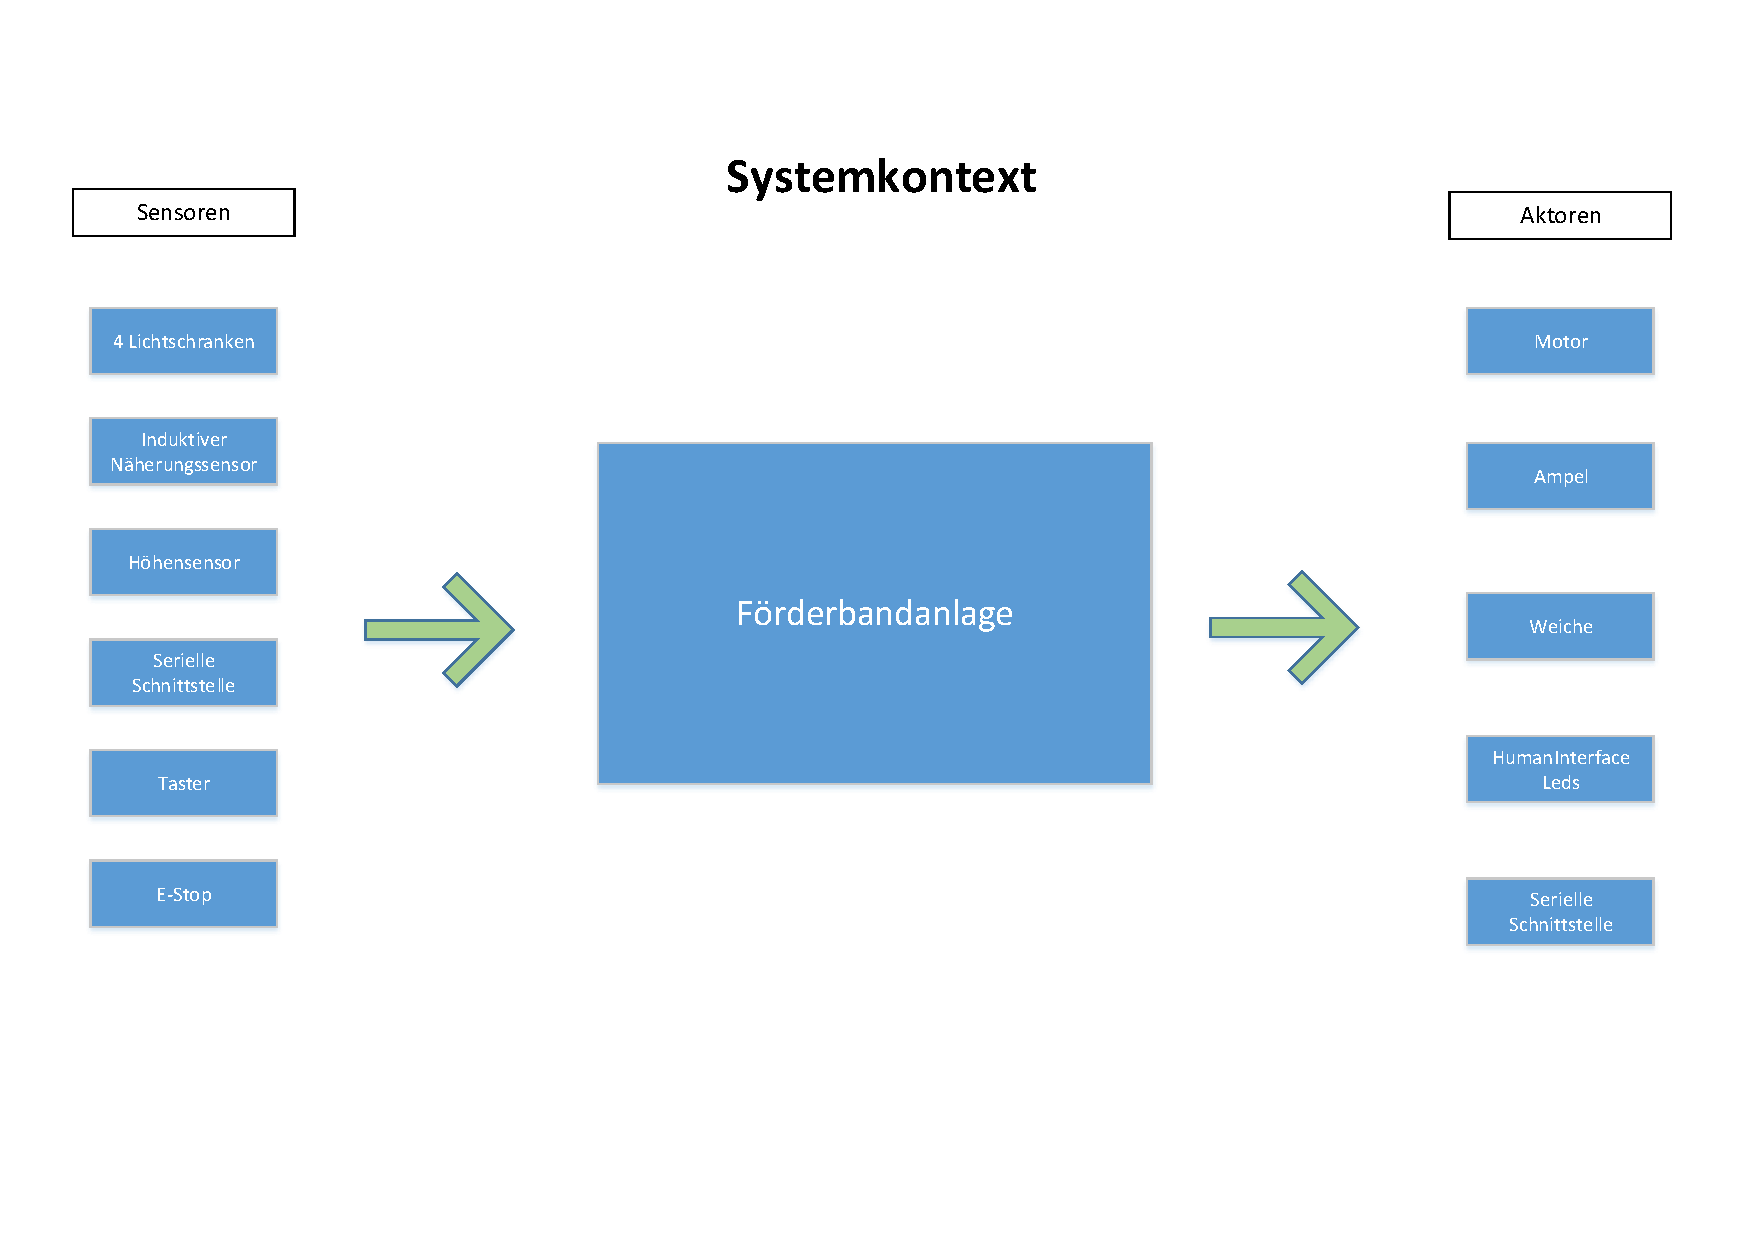
\includegraphics[scale=0.6]{images/Systemkontext.pdf}
    \caption{Systemgrenzen der Förderbandanlage mit Sensoren und Aktoren}
    \label{syskont}
\end{figure}

\begin{table}[H]
\center
    \begin{tabularx}{\textwidth}{|l|X|}
    \hline
    \textbf{Sensor}&\textbf{Aufgabe}\\
    \hline
    4 Lichtschranken&Erfassen, ob gerade ein Werkstück sich auf der Höhe der jeweiligen Lichtschranke befindet.\\
    \hline
    Induktiver Näherungssensor&Stellt fest, ob es sich um ein metallisches Werkstück handelt.\\
    \hline
    Höhensensor&Misst die Höhe des Werkstücks.\\
    \hline
    Serielle Schnittstelle&Ermöglicht den Empfang und das Senden von Datenpaketen anderer Nachbarsysteme.\\
    \hline
    Taster&Löst je nach Programmierung entsprechende Aktion aus.\\
    \hline
    E-Stop&Löst E-Stopp Aktion aus.\\
    \hline
    \end{tabularx}
    \caption{Sensoren und deren Aufgaben}
    \label{senstasks}
\end{table}

\begin{table}[H]
\center
    \begin{tabularx}{\textwidth}{|l|X|}
    \hline
    \textbf{Aktor}&\textbf{Aufgabe}\\
    \hline
    Motor&Treibt das band der Förderbandanlagen an.\\
    \hline
    Ampel&Signalisiert entsprechend anliegender Ereignisse.\\
    \hline
    Weiche&Dient zur Sortierung von Werkstücken.\\
    \hline
    HumanInterface Leds&Signalisieren dem Bediener Sensorereignisse\\
    \hline
    Serielle Schnittstelle&Ermöglicht das Versenden von Datenpaketen an andere Nachbarsysteme\\
    \hline
    \end{tabularx}
    \caption{Aktoren und deren Aufgaben}
    \label{acttasks}
\end{table}

\newpage

\subsection{Use Cases}

\begin{table}[h]
    \center
    \begin{tabularx}{\textwidth}{X}

    \begin{compactenum}[1.]
            \item \textbf{Flache Werkstücke aussortieren}
            \medskip

            Akteure: Mitarbeiter (legt die Werkstücke auf das Band), Höhenmessung, Weiche
            \medskip

            Auslösendes Ereignis: Höhenmessung erkennt das flache Werkstück.
            \medskip

            Kurzbeschreibung: Die flachen Werkstücke werden auf dem ersten und zweiten Förderband mit der Höhenmessung erkannt und über die jeweils eigene Weiche aussortiert.
            \bigskip

            \item \textbf{Werkstückdaten ausgeben}
            \medskip

            Akteure: letzte Lichtschranke, Display, zweites Förderband
            \medskip

            Auslösendes Ereignis: Die letzte Lichtschranke des zweiten Förderbandes wird durchquert.
            \medskip

            Kurzbeschreibung: Wenn ein Werkstück das Ende vom zweiten Förderband erreicht, werden die Werkstückdaten auf dem Display ausgegeben.
            \bigskip

            \item \textbf{Ausgabe der Werkstücke auf drittem Förderband in der richtigen Reihenfolge}
            \medskip

            Akteure: Lichtschranke, Mitarbeiter (nimmt die Werkstücke in Empfang), Weiche
            \medskip

            Auslösendes Ereignis: Es sind die drei richtigen Werkstücke auf dem dritten Förderband vorhanden.
            \medskip

            Kurzbeschreibung: Auf dem dritten Förderband werden jeweils drei Werkstücke gebündelt in der richtigen Reihenfolge ($\text{Bohrung oben ohne Metall}\rightarrow \text{Bohrung oben ohne Metall}\rightarrow \text{Bohrung oben mit Metall}$) ausgegeben.
        \end{compactenum}
    \end{tabularx}
%\caption{Tabellenunterschrift}
\label{ucs}
\end{table}

\newpage

\section{Design}
Im Designkapitel sind Systemarchitektur, Datenmodellierung und Verhaltensmodellierung der Förderbänder enthalten.

\subsection{Systemarchitektur}
Die Systemarchitektur setzt sich aus den internen Architekturen der drei Förderbänder und der Architektur des Gesamtsystems, welche die Schnittstellen der drei Förderbänder zueinander darstellt, zusammen.

\subsubsection{Förderband intern}

\begin{figure}[H]
\centering 
    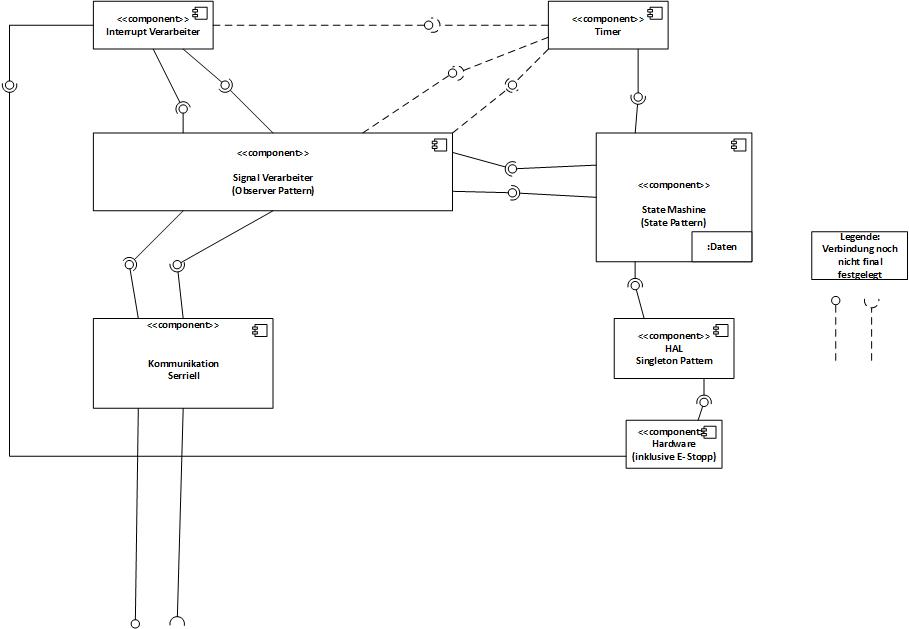
\includegraphics[scale=0.7]{images/SW_Architektur/Foerderband.jpg}
    \caption{Interne Systemarchitektur eines Förderbandes}
    \label{archintern}
\end{figure}

\begin{table}[H]
\center
    \begin{tabularx}{\textwidth}{|l|X|}
        \hline
        \textbf{Komponente}&\textbf{Aufgabe}\\
        \hline
        Interrupt Verarbeiter&Verarbeitet Interrupts aus Timer, Signal Verarbeiter und Hardware.\\
        \hline
        Timer&Dient zur Zeiterfassung und Überprüfung von verschwundenen oder fehlerhaft hinzugefügten 
        Werkstücken.\\
        \hline
        Signal Verarbeiter&Verarbeitet Signale aus Interrupt Verarbeiter, Timer, Statemachine und Kommunikation seriell.\\
        \hline
        Statemachine&Steuert den logischen Ablauf.\\
        \hline
        Kommunikation seriell&Bildet die Schnittstelle zwischen Förderband und Gesamtsystem.\\
        \hline
        HAL&Hardwareabstraktionsschicht zur Ansteuerung der Komponenten eines Förderbandes.\\
        \hline
        Hardware&Hardware des Förderbandes\\
        \hline
        \end{tabularx}
    \caption{Aufgaben der Komponenten eines Förderbandes}
    \label{archinterntcomp}
\end{table}

\newpage

\subsubsection{Gesamtsystem}

\begin{figure}[H]
\centering 
    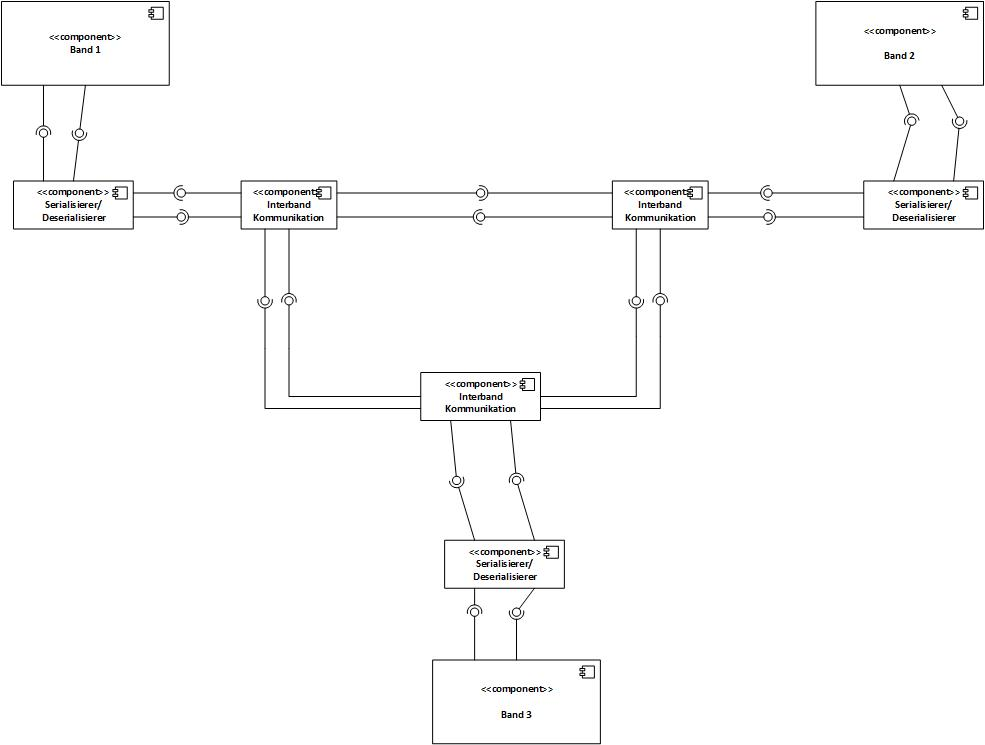
\includegraphics[scale=0.60]{images/SW_Architektur/Gesamtsystem.jpg}
    \caption{Systemarchitektur des Gesamtsystems}
    \label{archtotal}
\end{figure}

\begin{table}[H]
\center
    \begin{tabularx}{\textwidth}{|l|X|}
        \hline
        \textbf{Komponente}&\textbf{Aufgabe}\\
        \hline
        Band 1&Erstes Förderband, welches die Sortierung entsprechend der Reihung durchführt.\\
        \hline
        Band 2&Zweites Förderband, welches die Sortierung entsprechend der Reihung durchführt mit anschließender Konsolenausgabe von Werkstückdaten.\\
        \hline
        Band 3&Drittes Förderband, welches die Gruppierung der Werkstücke übernimmt und anschließend übergibt.\\
        \hline
        Serialisierer/Deserialisierer&Serialisiert bzw. deserialisiert Datenpakete zur Kommunikation.\\
        \hline
        Interband Kommunikation&Empfängt bzw. versendet serialisierte Datenpakete.\\
        \hline
        \end{tabularx}
    \caption{Aufgaben der Komponenten des Gesamtsystems}
    \label{archtotalcomp}
\end{table}

%\newpage

\subsection{Datenmodellierung}
Die Modellierung der Klassen und dessen Methoden sind mithilfe von UML-Diagrammen realisiert.
\subsubsection{HAL}
Mit der Klasse HAL werden die Hardwarekomponenten eines Förderbandes angesteuert. Dabei wird jede Hardwarekomponente nach dem Singleton-Pattern instanziiert. Die nachfolgende Abbildung \hyperref[sec:umlhal]{5} stellt alle Klassen zur HAL mit ihren Methoden dar.

\newpage

%Abbildungszähler
\newcounter{imgcounter}
\setcounter{imgcounter}{4}

\stepcounter{imgcounter}
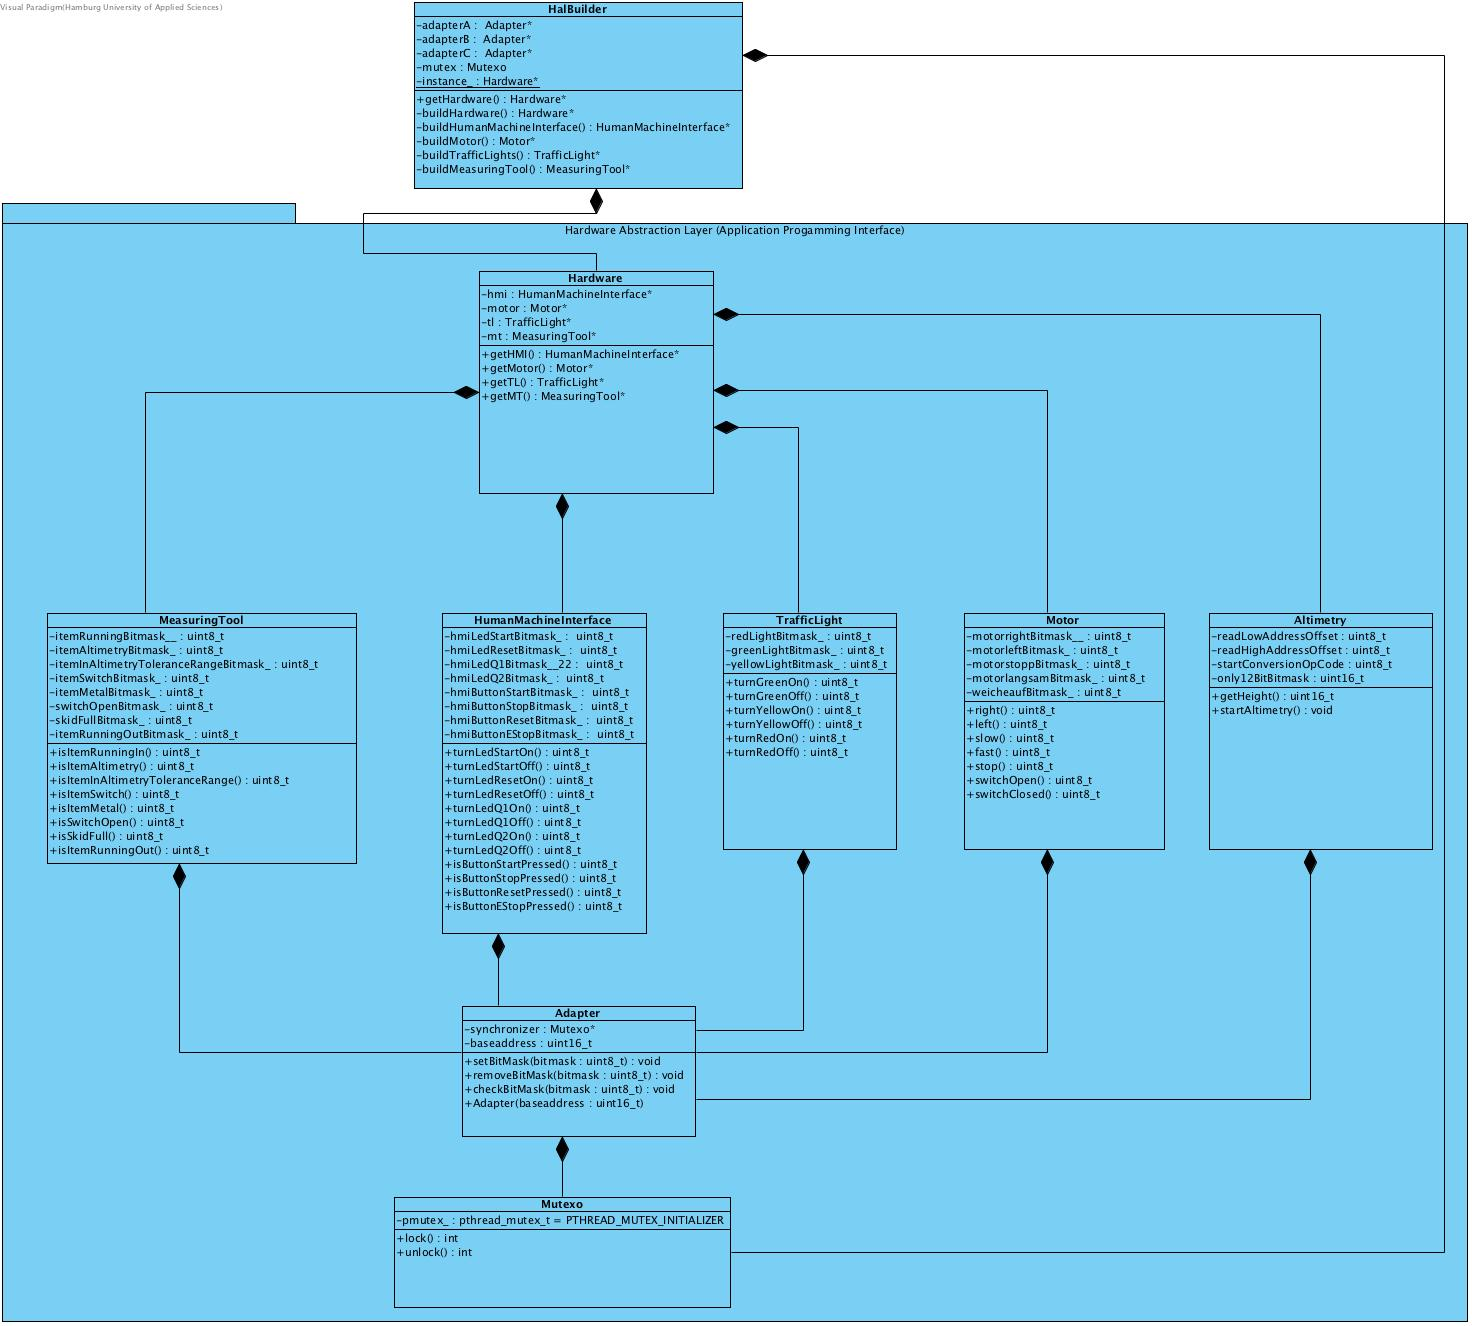
\includepdf[scale=1, landscape=true, pages=1,offset=0 0, pagecommand=
\vspace*{25cm}
\hspace*{3cm} Abbildung \theimgcounter : UML-Diagramm zur HAL]{images/HAL_UML.jpg}\label{sec:umlhal}
\newpage

\subsection{Zeitmessung}
Auf dem ersten und zweiten Förderband müssen Zeitmessungen durchgeführt werden, um Zeiten zu erfassen, mit denen im Normalbetrieb unsachgemäß hinzugefügte Werkstücke oder das Verschwinden von Werkstücken erkannt werden kann.

\subsubsection{Vorbedingungen}
Für die Zeitmessung muss die gleiche Implementation der Förderbandlogik ablaufen, die auch im Normalbetrieb für die beiden ersten Förderbänder ablaufen wird, wobei die Höhenmessung ausgelassen wird und das Werkstück bedingungslos durchgelassen wird. Falls in der Routine Geschwindigkeitsänderungen des Bandes vorliegen, müssen diese jedoch miteinbezogen werden.
Da ein Werkstück am Anfang des ersten Förderbändes unterschiedlich hinzugefügt werden kann (siehe Abbildung \hyperref[sec:Messpunkte]{6}) und der Timer eine relativ hohe Zeitauflösung hat, müssen \textbf{best} und \textbf{worst case} Zeiten ermittelt werden. 

\subsubsection{Ausführung}
Für den \textbf{\textcolor{ForestGreen}{best case}} wird das Werkstück beim Hinzufügen von der ersten Lichtschranke aus gesehen am \textbf{\textcolor{ForestGreen}{linken Rand}} der Führung angelegt, während beim \textbf{\textcolor{OrangeRed}{worst case}} am \textbf{\textcolor{OrangeRed}{rechten Rand}} angelegt werden muss. Dabei muss das Werkstück die erste Lichtschranke \textbf{LS\_A} auch unterbrechen, was auch im Normalbetrieb beim Hinzufügen weiterer Werkstücke beachtet werden muss! Die Zeitmessung beginnt, nachdem das Werkstück die Lichtschranke am Anfang nicht mehr unterbricht. Unterbricht das Werkstück die nachfolgenden Lichtschranken, wird jeweils die Zeit gestoppt. Die nachfolgende Abbildung \hyperref[sec:Messpunkte]{6} zeigt wann die Zeiten $t_0, t_H, t_W$ und $t_E$ erfasst werden.

\stepcounter{imgcounter}
\begin{figure}[h]
\centering 
    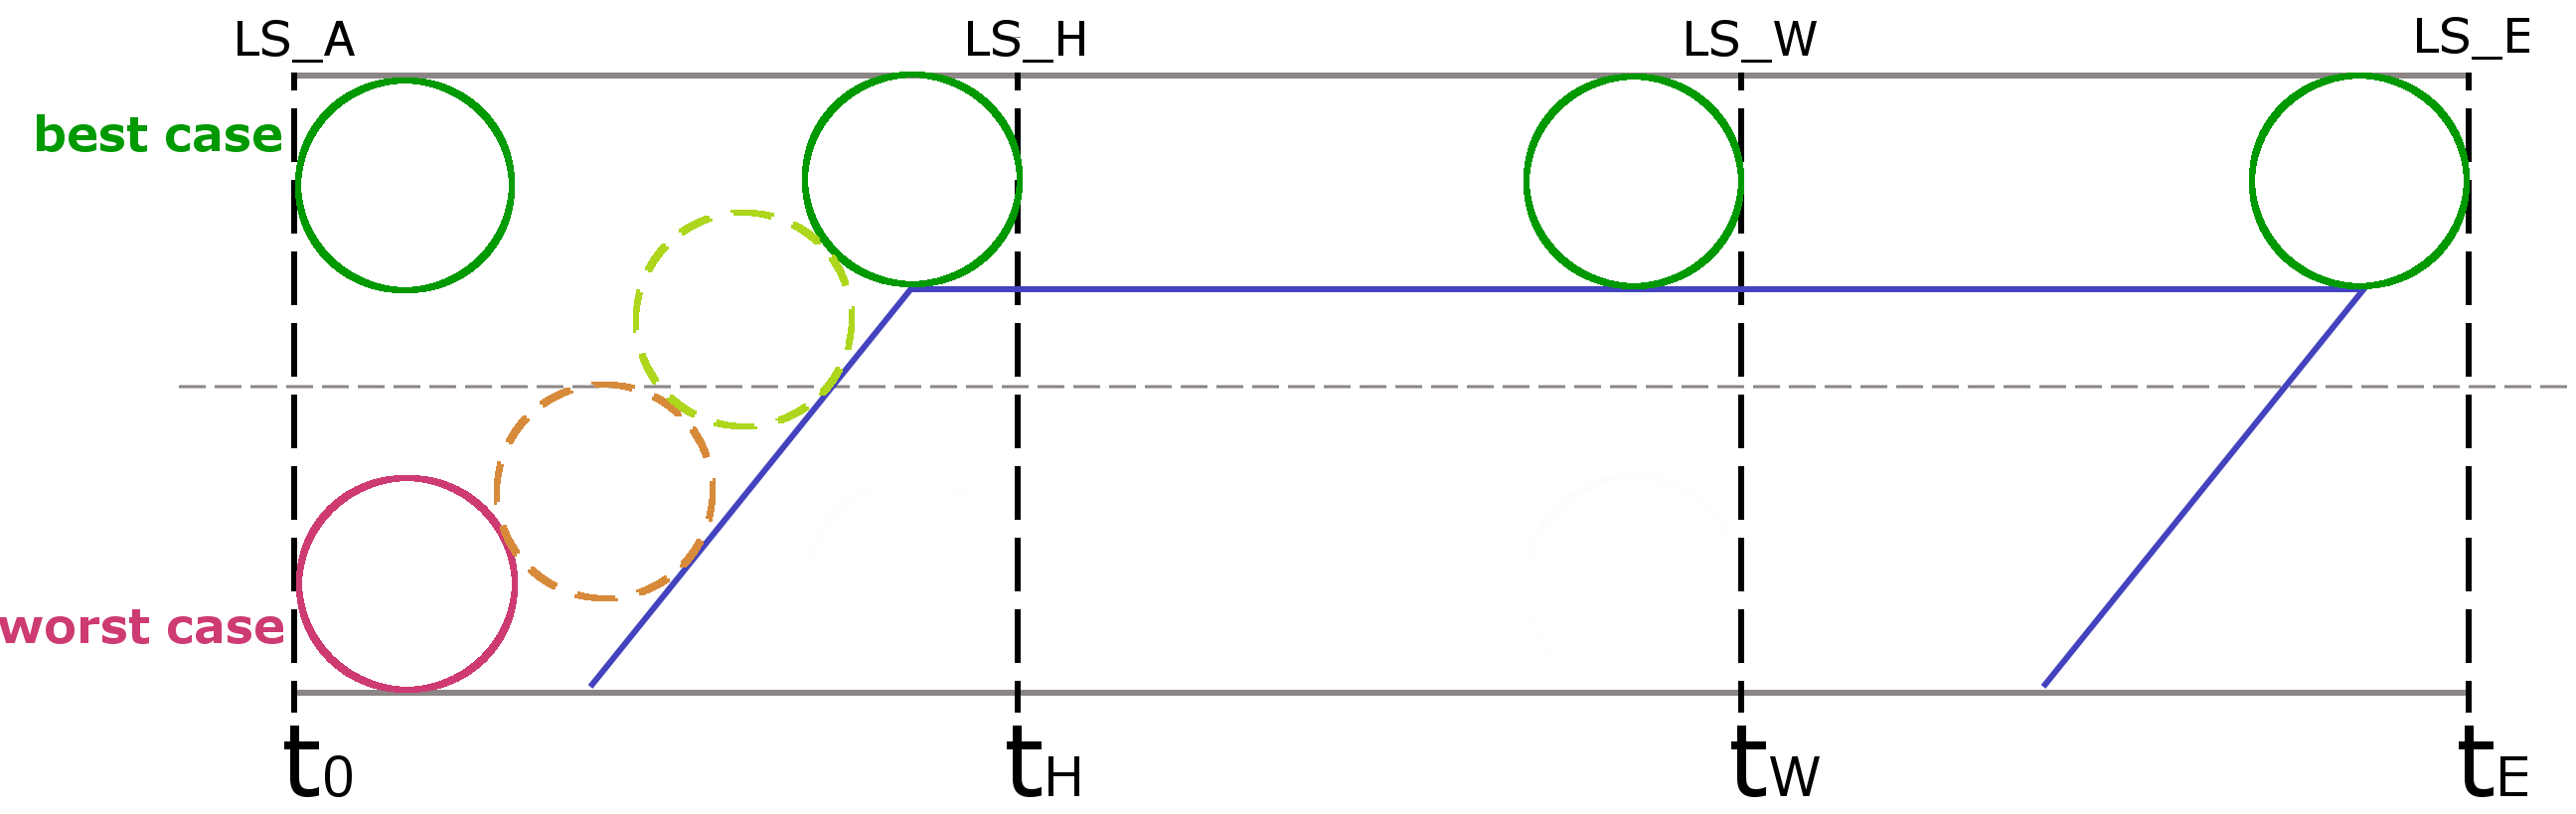
\includegraphics[scale=0.6]{images/Zeitmessung_Platzierung.png}
    \caption*{Abbildung \theimgcounter : Stoppen der Zeit an den Lichtschranken: \textit{LS\_A, LS\_H, LS\_W, LS\_E}}
    \label{sec:Messpunkte}
\end{figure}

\begin{table}[H]
\centering
    \begin{tabularx}{\textwidth}{|X|X|}
        \hline
        \textbf{Abkürzung}&\textbf{Beschreibung}\\
        \hline
        LS\_A & Lichtschranke-Anfang\\
        \hline
        LS\_H & Lichtschranke-Höhenmessung\\
        \hline
        LS\_W & Lichtschranke-Weiche\\
        \hline
        LS\_E & Lichtschranke-Ende\\
        \hline
    \end{tabularx}
\caption{Abkürzende Lichtschrankenbezeichnung}
\label{lbdesc}
\end{table}

\noindent Auf der nachfolgenden Seite sind die endlichen Automaten in Abbildung \hyperref[sec:timemeasure]{7} zur Zeitmessung abgebildet.
\stepcounter{imgcounter}
\includepdf[scale=0.9,pages=5, landscape=true, offset=0 0, pagecommand=
\vspace*{25cm}
\hspace*{0.5cm} Abbildung \theimgcounter : FSM zur Zeitmessung für schnellen und langsamen Bandlauf]{FSM/Statemachines.pdf}\label{sec:timemeasure}

\newpage

\subsection{Verhaltensmodellierung}
Das Verhalten der drei Förderbänder ist mithilfe von hierarchischen Zustandsautomaten realisiert. Die Abbildungen \hyperref[sec:hsm1]{8}, \hyperref[sec:hsm2]{9} und \hyperref[sec:hsm3]{10} auf den folgenden Seiten bilden die Förderbänder 1, 2 und 3 ab. Anschließend sind in Abbildung \hyperref[sec:hsm4]{11} die Zustandsautomaten zu den Förderbandkomponenten und dem Timer sowie zum Timeout zu sehen. Die Förderbandkomponenten Motor und Weiche sowie der Timer sind für jedes Förderband auch in Software nur \textbf{einmal} vorhanden. Der Timeout Automat wird jedoch für jeden einzelnen Puck einmal erstellt und verwendet.

\newpage
\stepcounter{imgcounter}
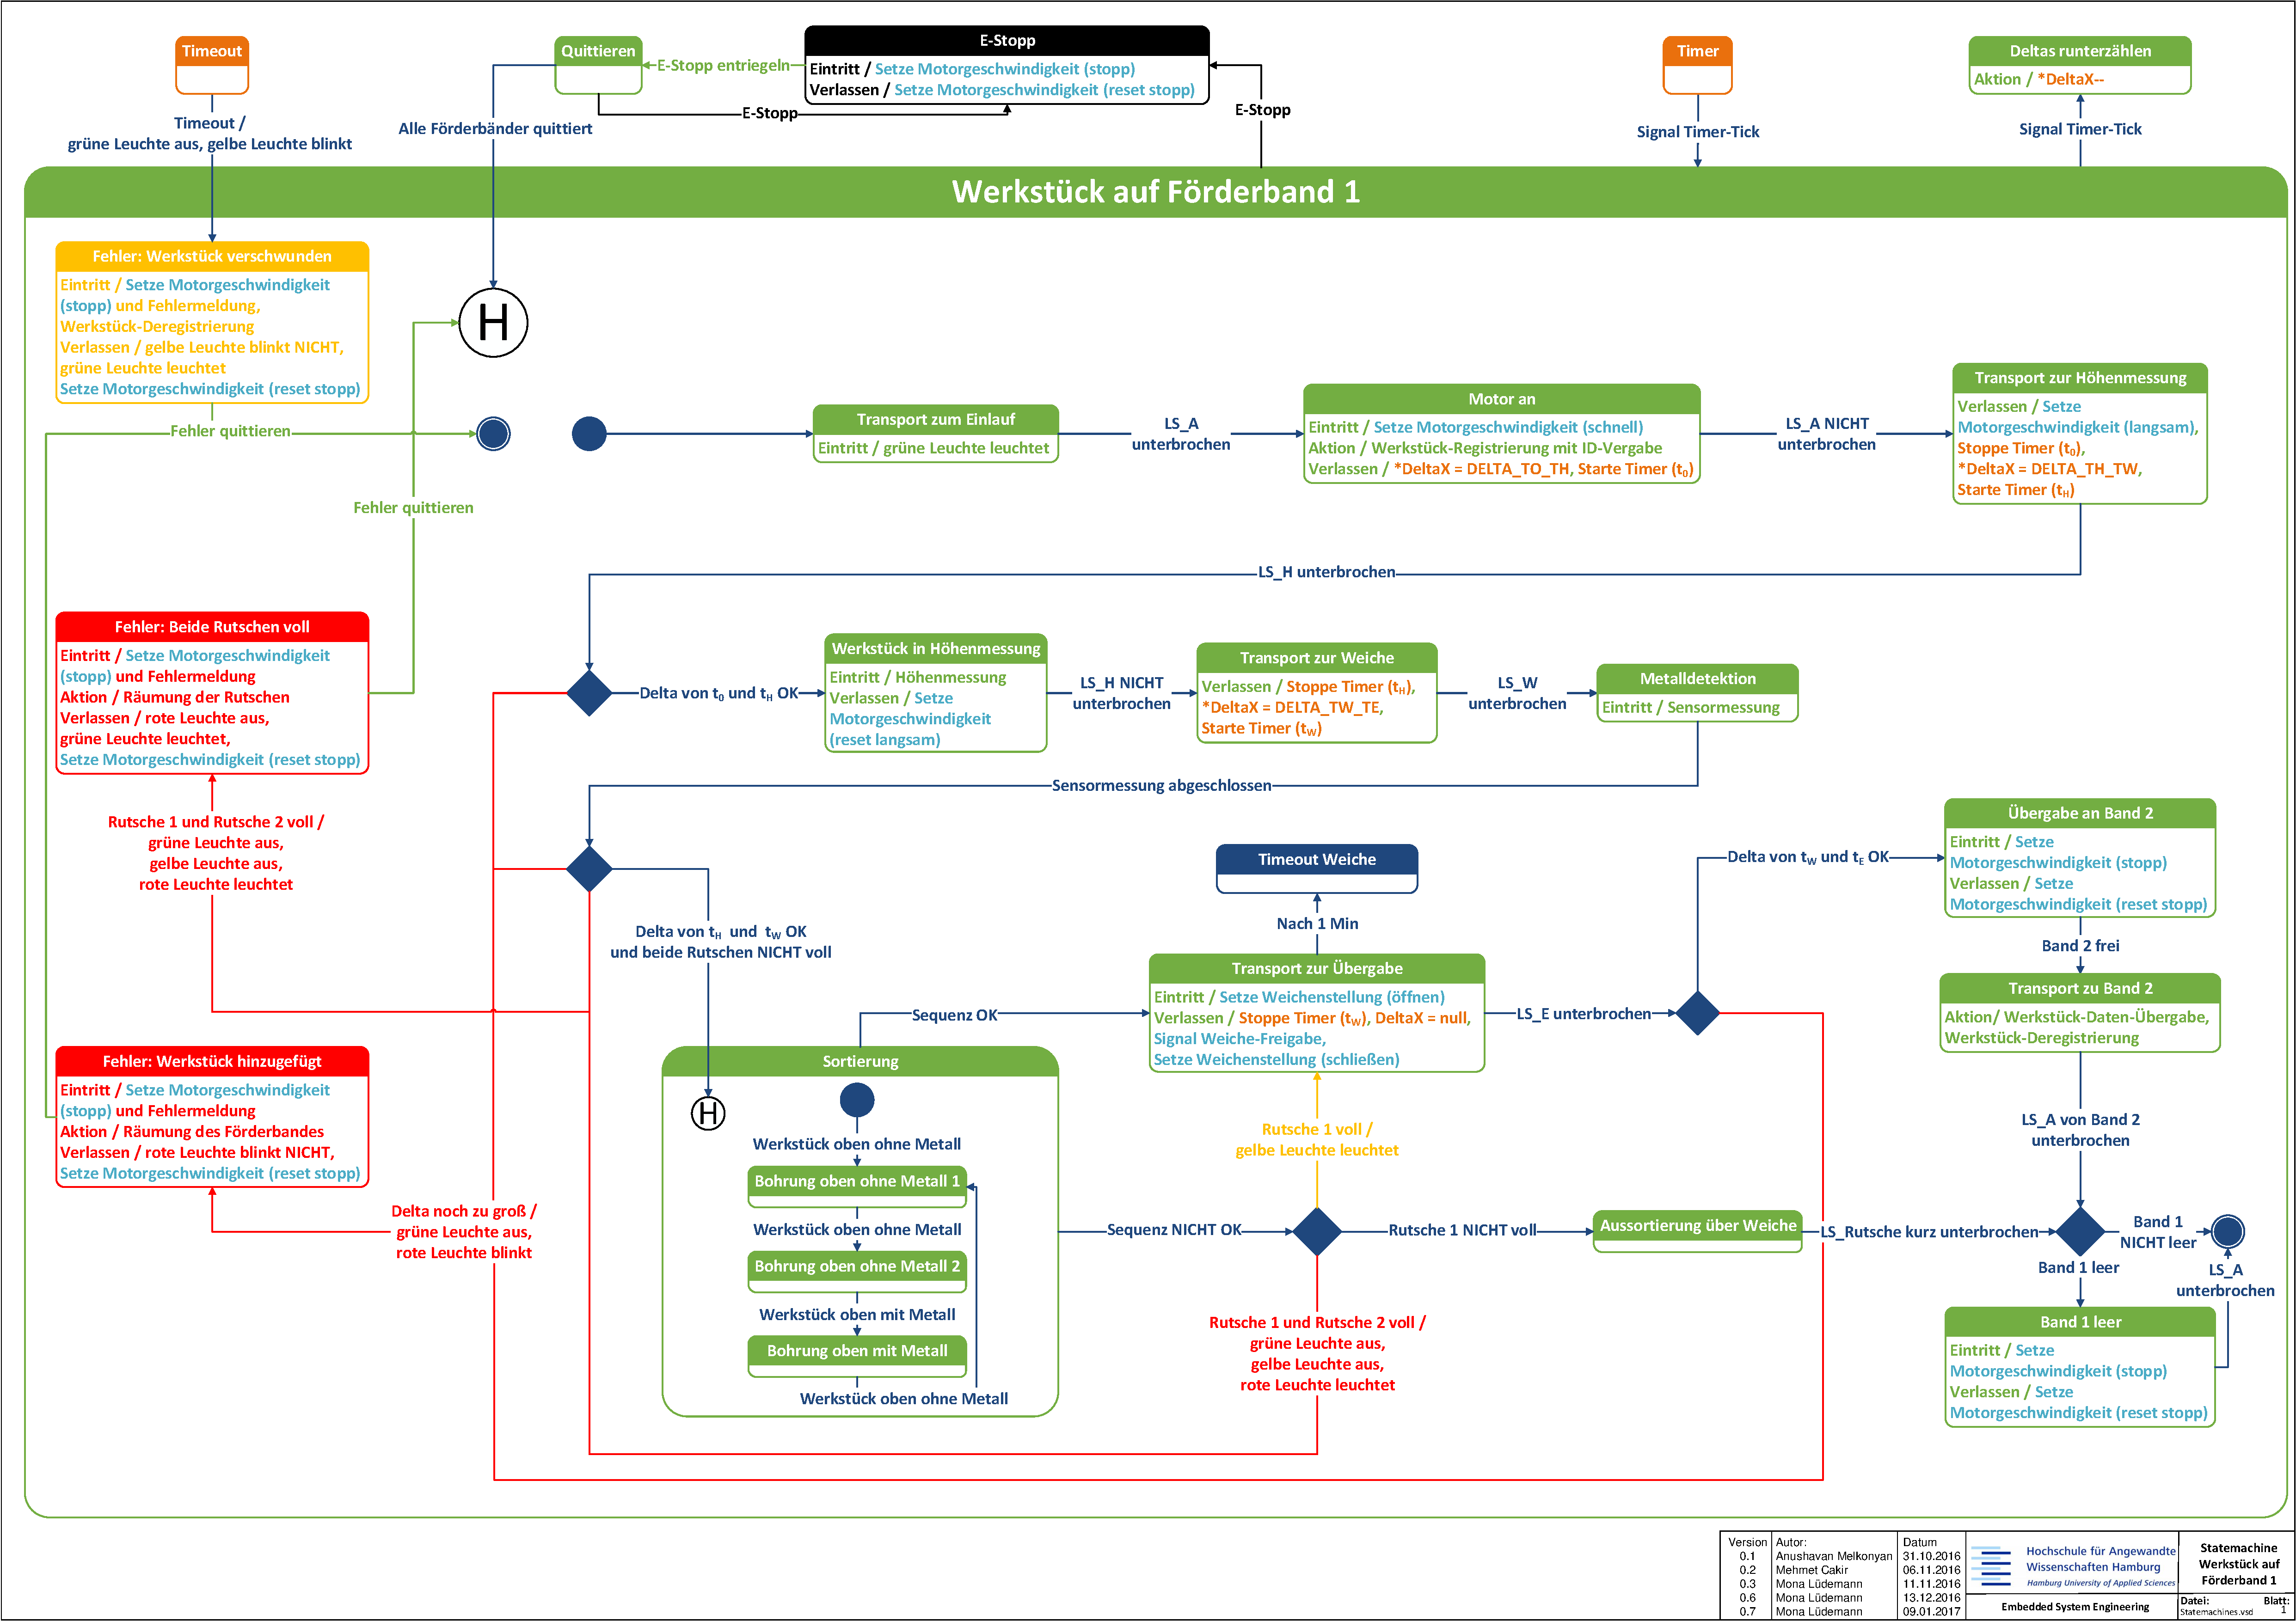
\includepdf[scale=0.87,pages=1, landscape=true, offset=0 13, pagecommand=
\vspace*{25cm}
\hspace*{3cm} Abbildung \theimgcounter : HSM zu Förderband 1]{FSM/Statemachines.pdf}\label{sec:hsm1}

\newpage
\stepcounter{imgcounter}
\includepdf[scale=0.86,pages=2, landscape=true, offset=0 15, pagecommand=
\vspace*{24.9cm}
\hspace*{3cm} Abbildung \theimgcounter : HSM zu Förderband 2]{FSM/Statemachines.pdf}\label{sec:hsm2}

\newpage
\stepcounter{imgcounter}
\includepdf[scale=0.86,pages=3, landscape=true, offset=0 13, pagecommand=
\vspace*{24.9cm}
\hspace*{3cm} Abbildung \theimgcounter : HSM zu Förderband 3]{FSM/Statemachines.pdf}\label{sec:hsm3}

\newpage
\stepcounter{imgcounter}
\includepdf[scale=0.86,pages=4, landscape=true, offset=0 13, pagecommand=
\vspace*{24.9cm}
\hspace*{3cm} Abbildung \theimgcounter : \text{HSM zu Motor, Weiche, Timer und Timeout}]{FSM/Statemachines.pdf}\label{sec:hsm4}

\newpage

\section{Implementierung}
Für die Implementierung der Software, welche die Logik der Werkstück-Sortieranlage realisiert, ist das Reagieren auf Änderungen an Sensoren sowie die Kommunikation unter den Förderbändern essentiell.

\subsection{Serielle Schnittstelle}
\begin{figure}[H]
\centering 
    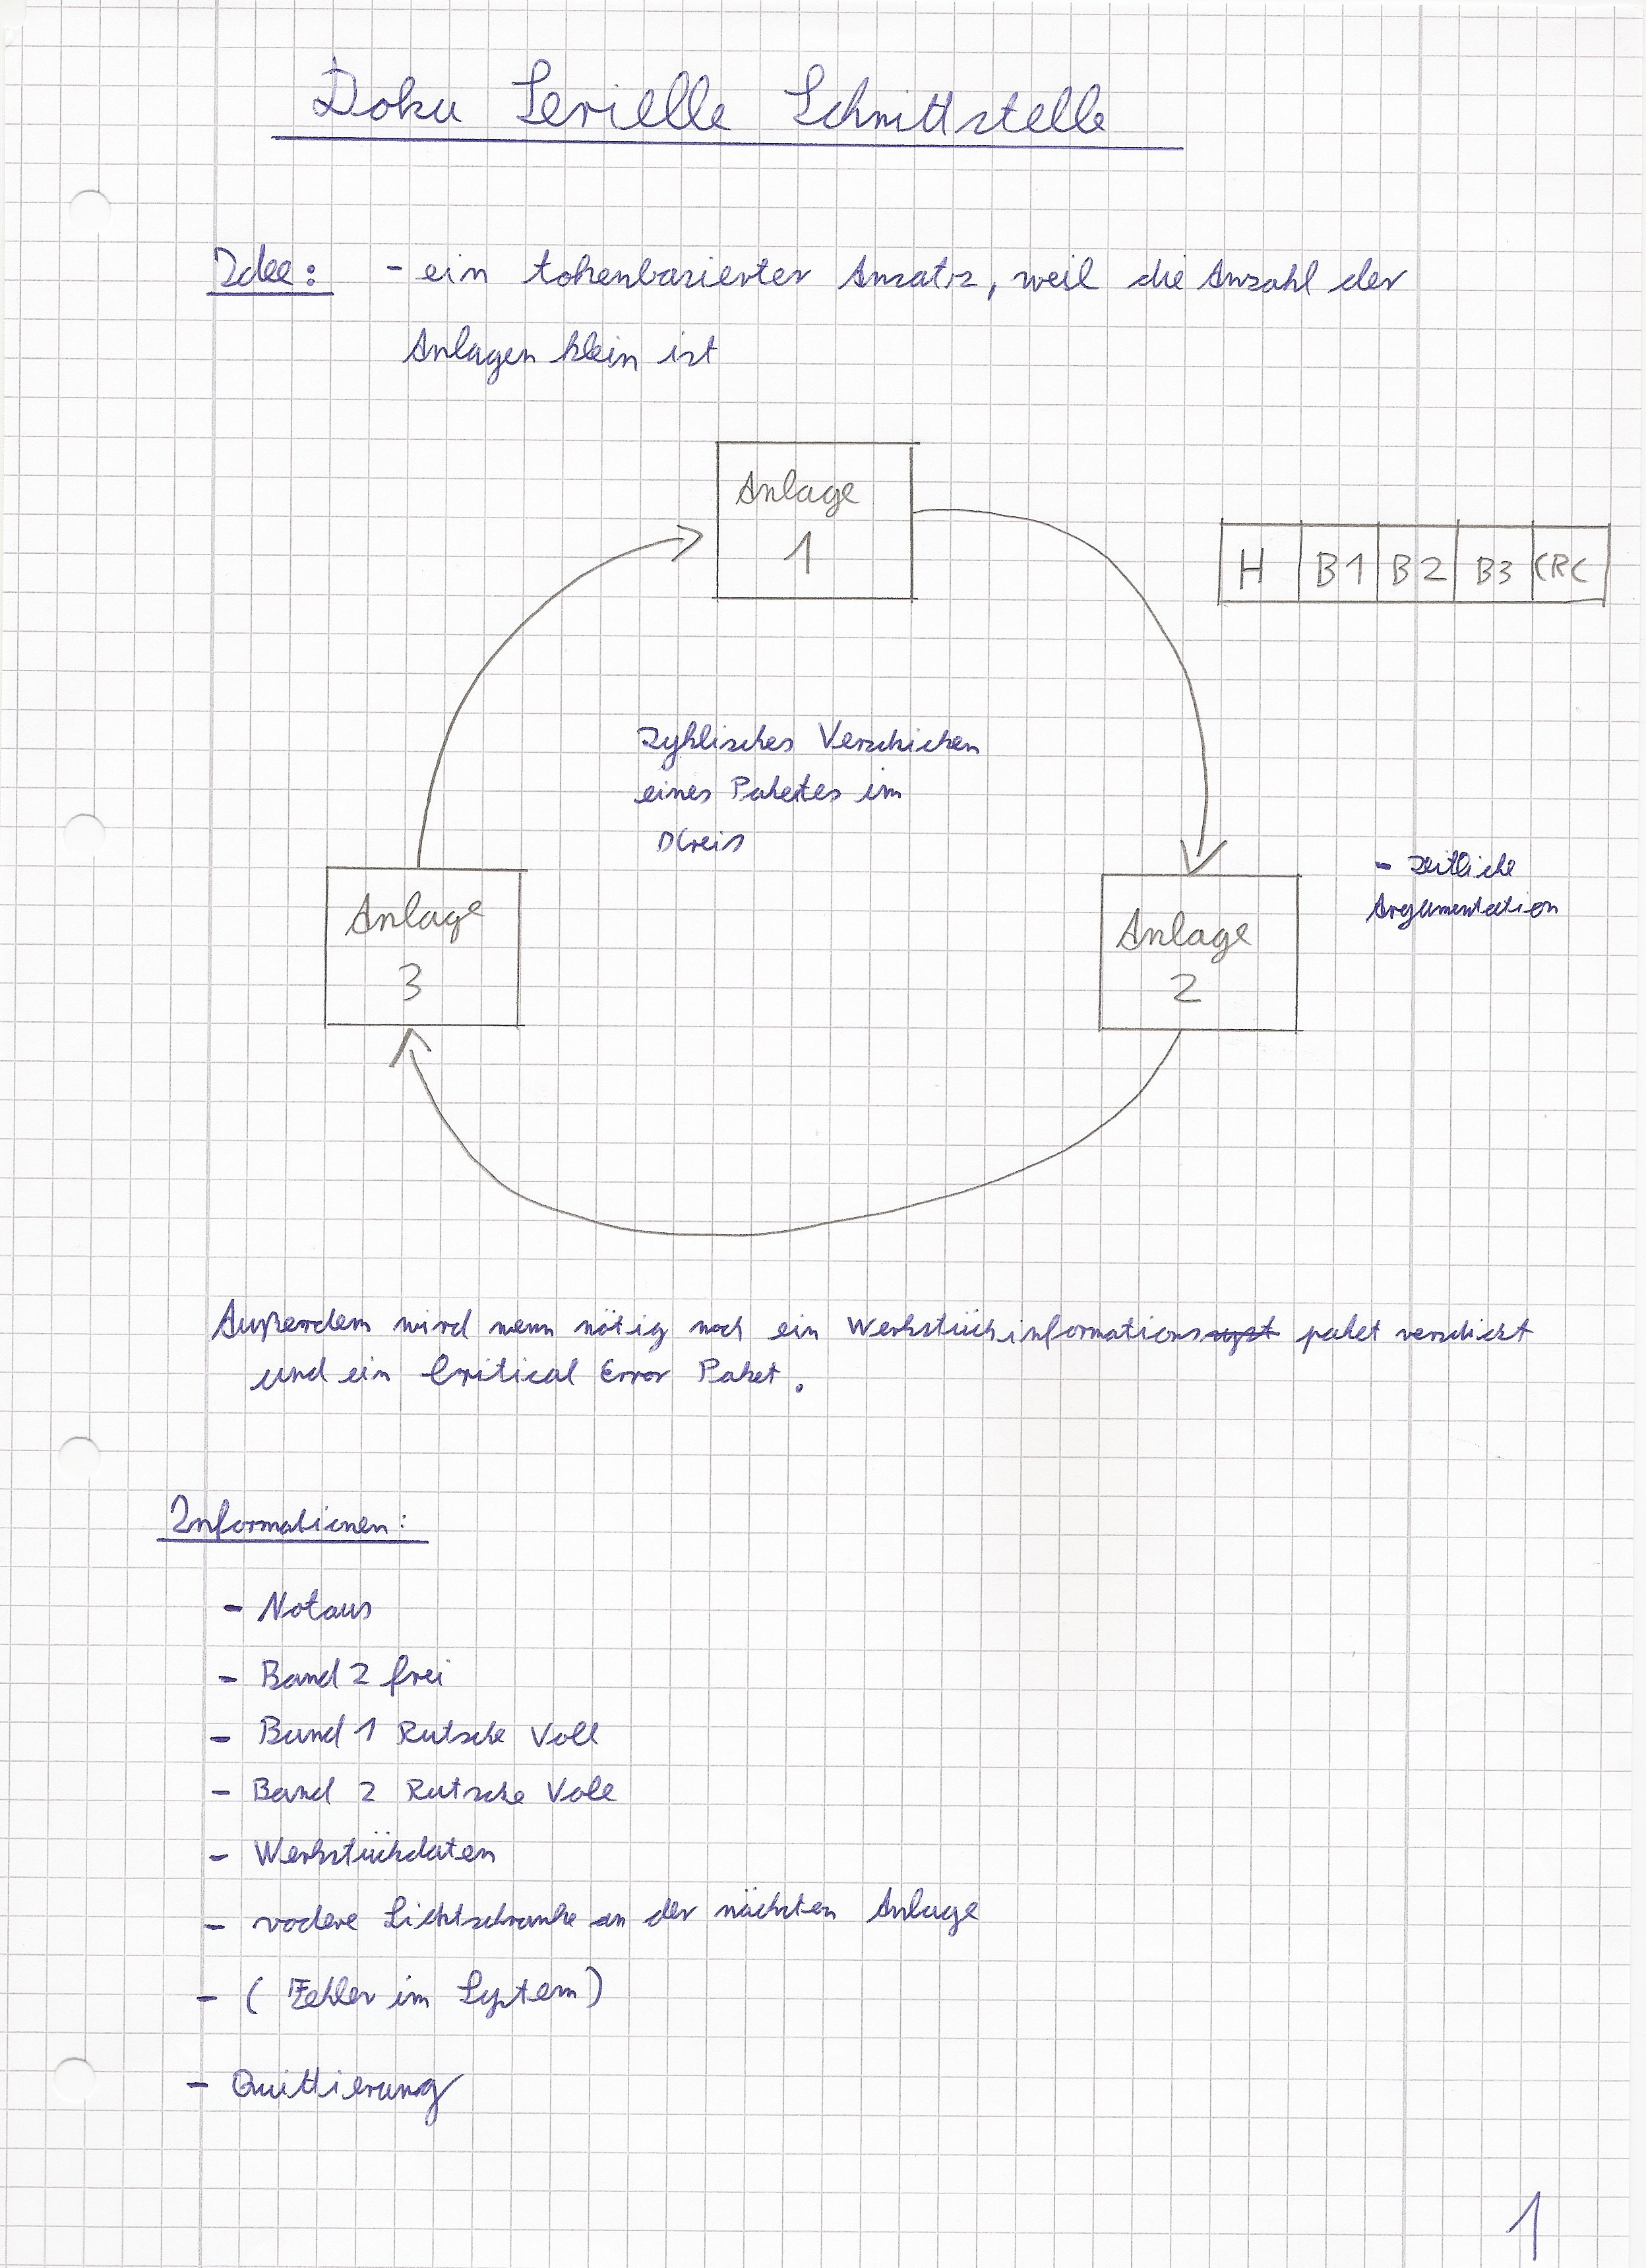
\includegraphics[scale=0.69]{SI/si1.jpg}
    \label{si1}
\end{figure}

\newpage

\begin{figure}[H]
\centering 
    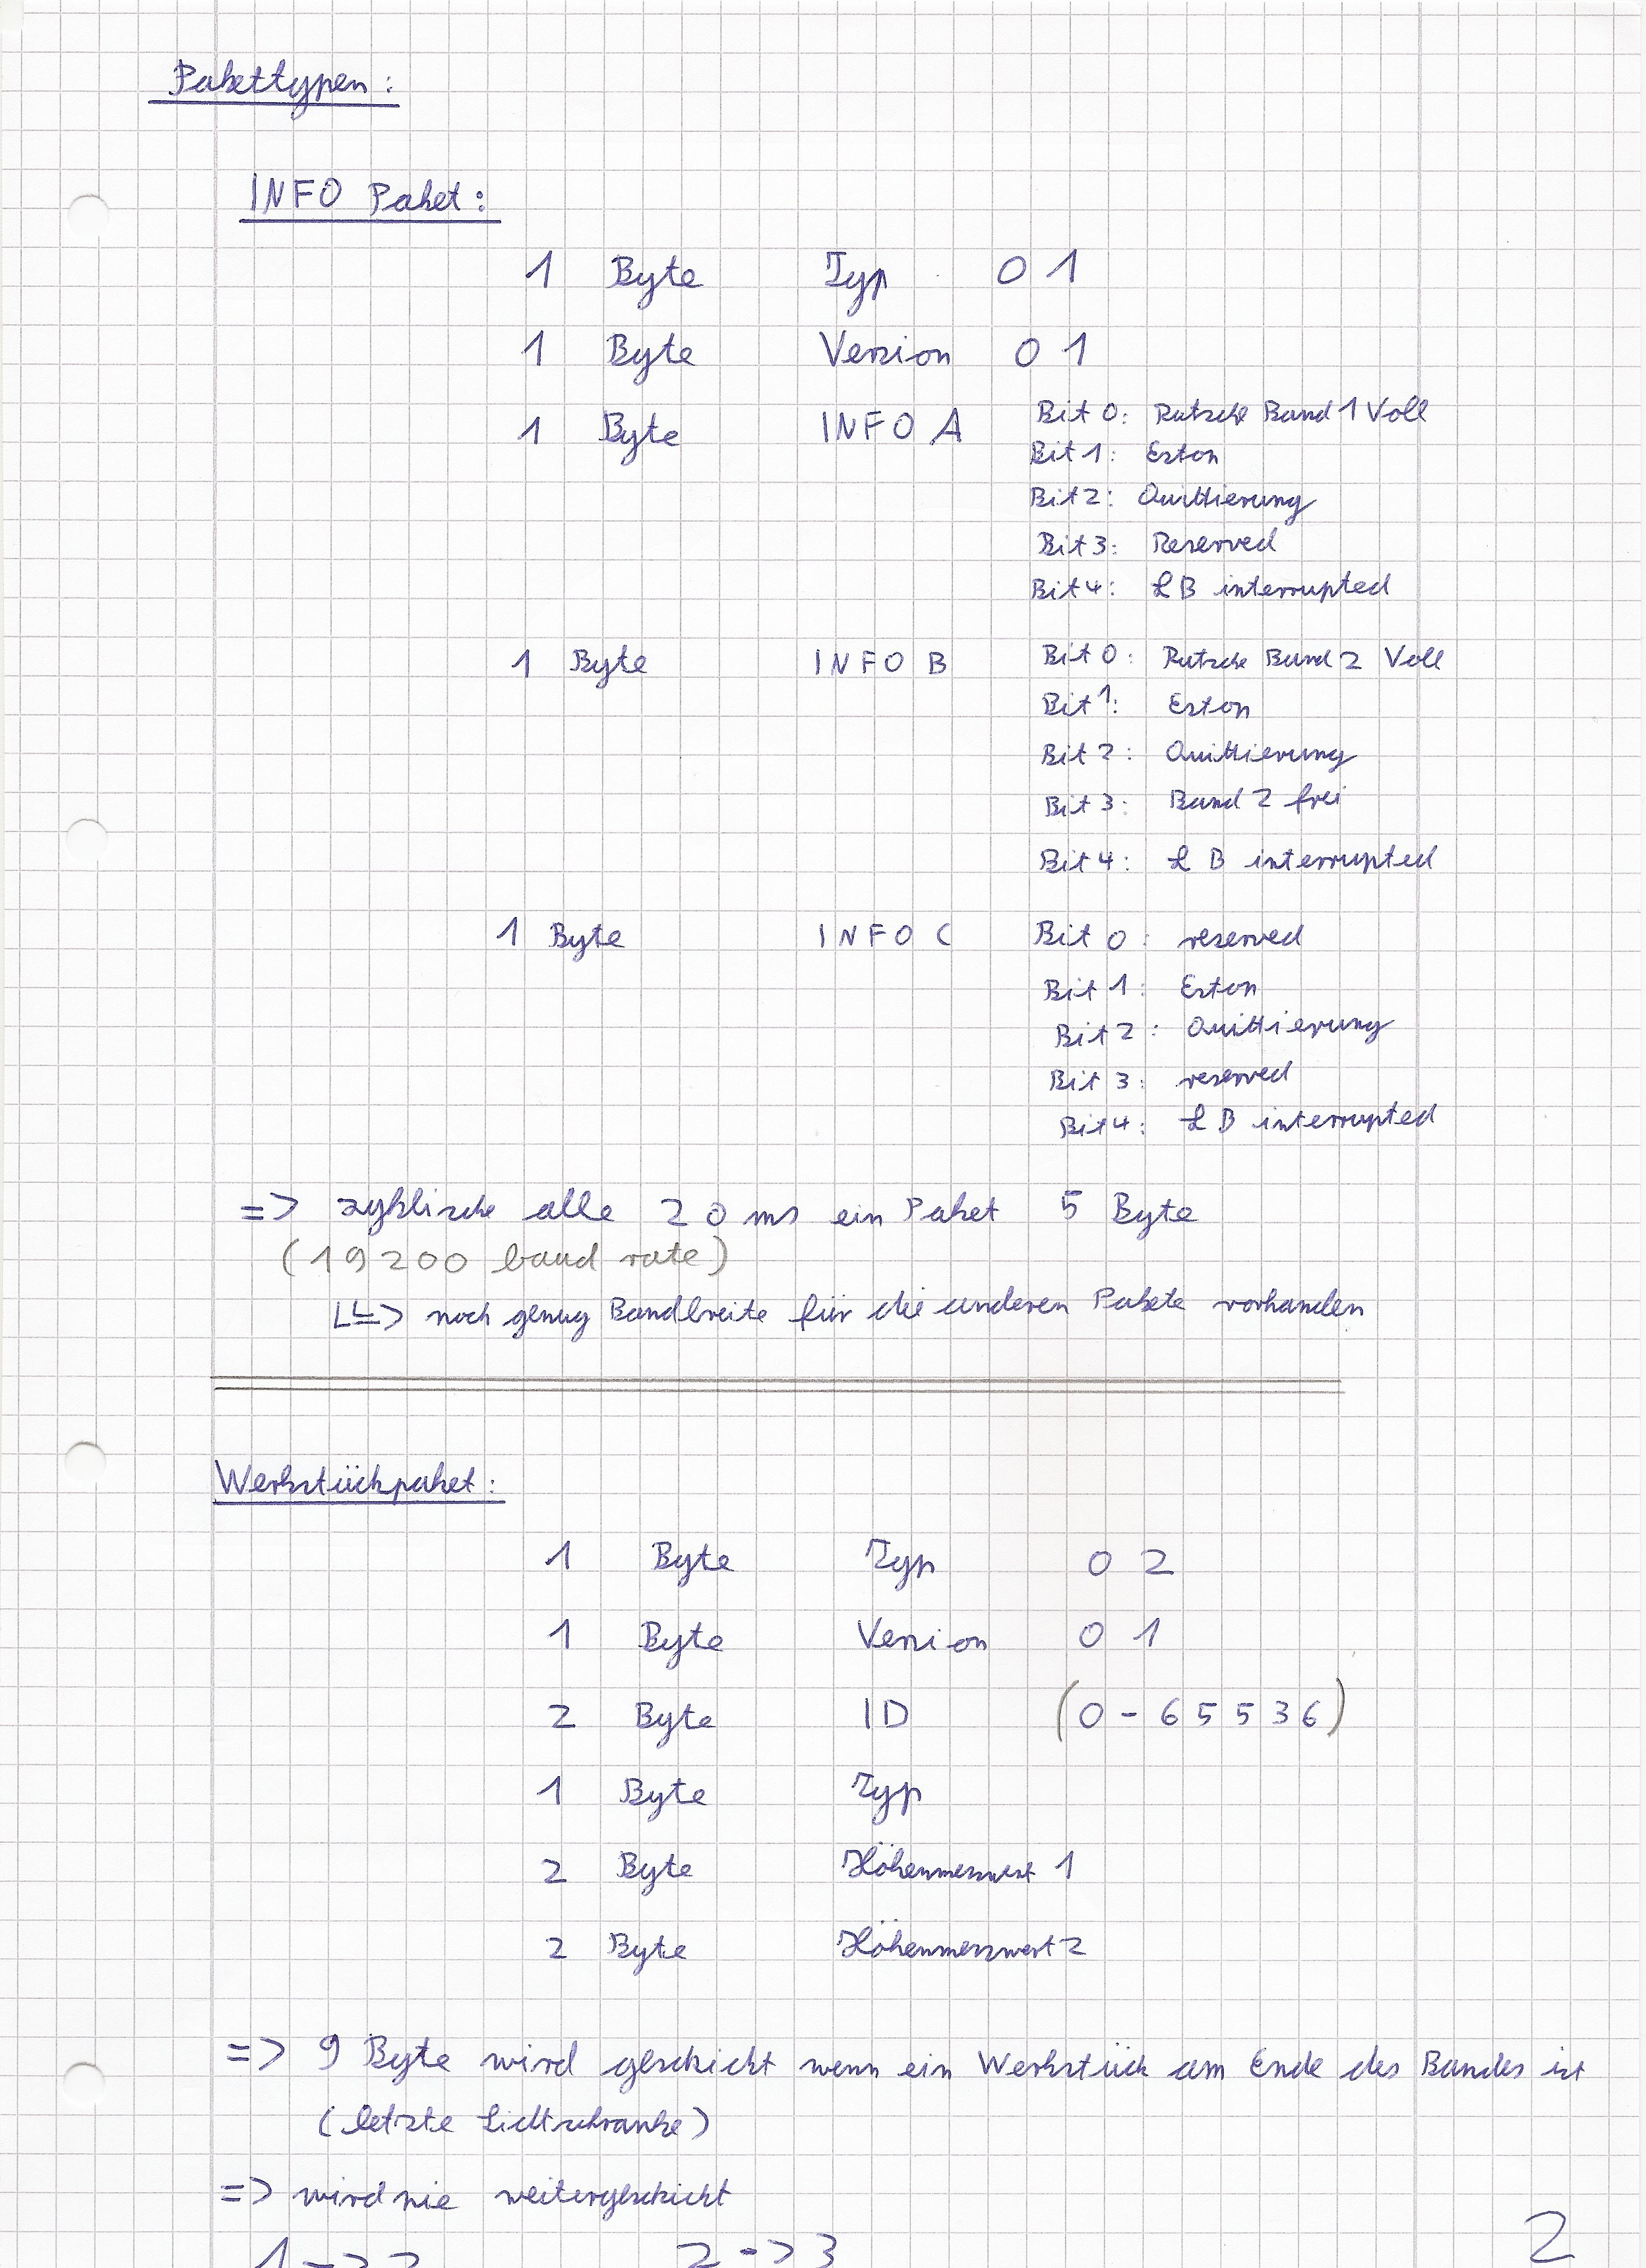
\includegraphics[scale=0.8]{SI/si2.jpg}
    \label{si2}
\end{figure}

\newpage

\begin{figure}[H]
\centering 
    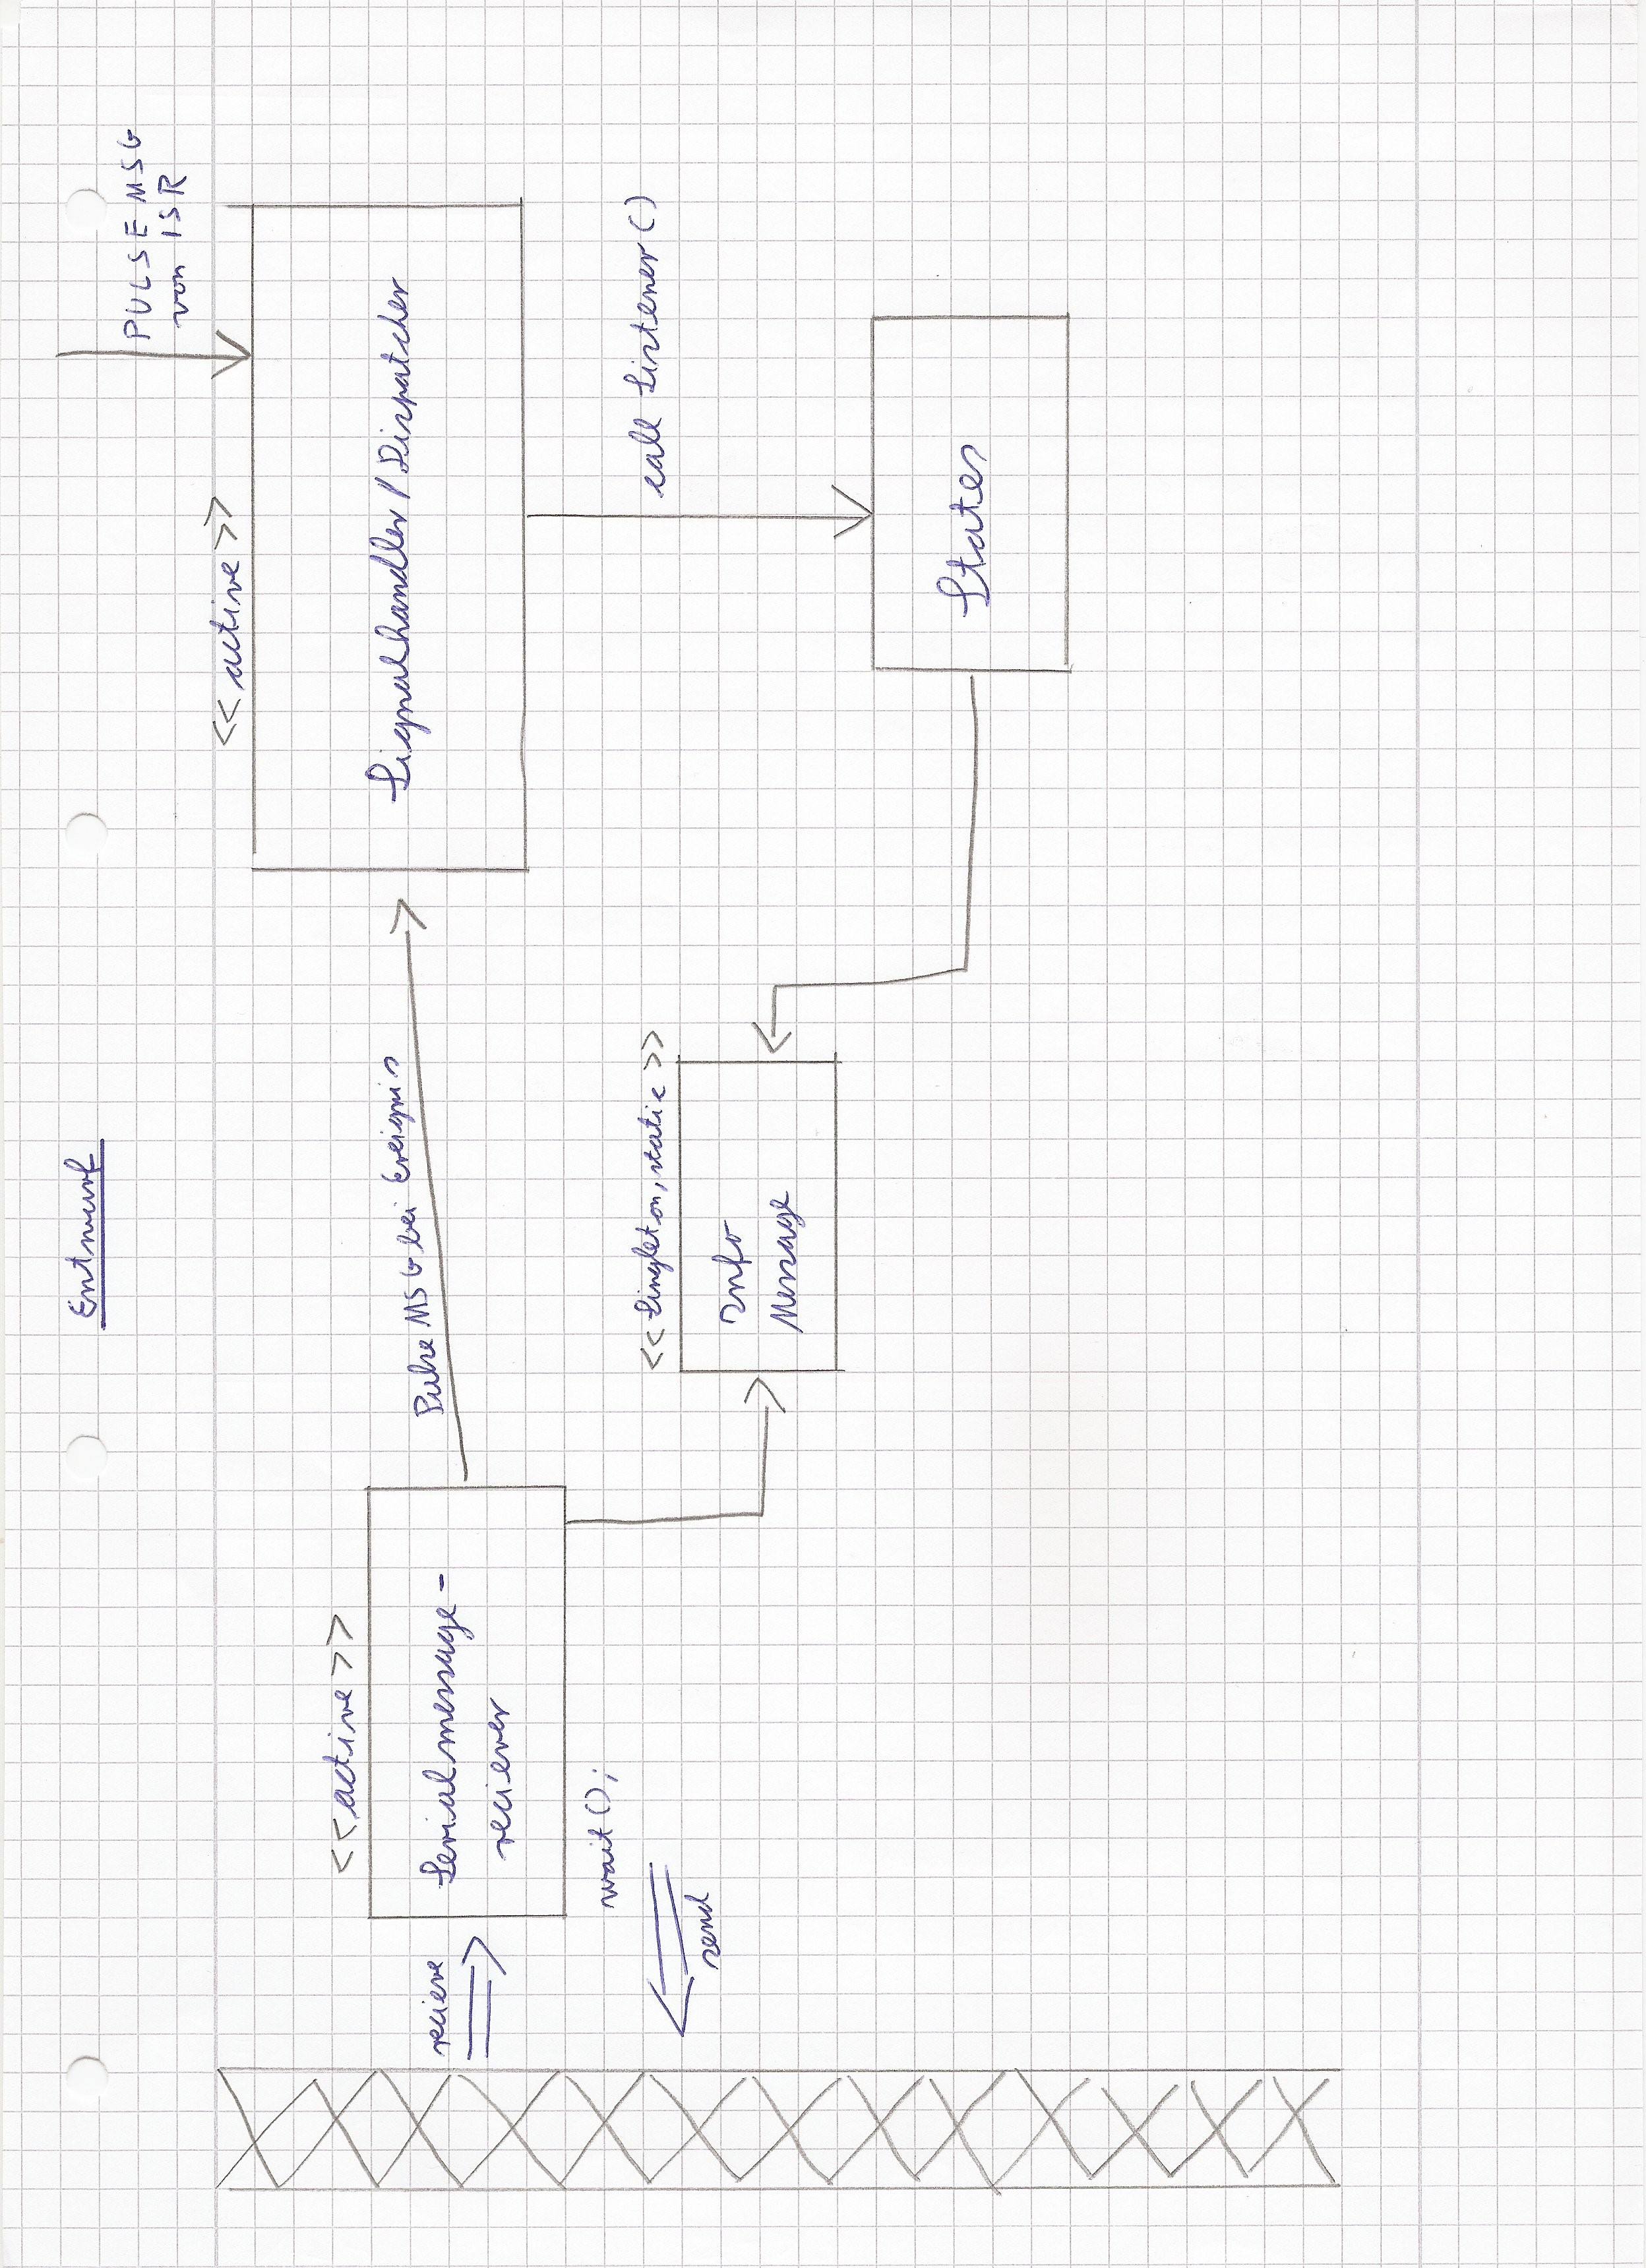
\includegraphics[scale=0.8]{SI/si3.jpg}
    \label{si3}
\end{figure}

\newpage

\subsection{ISR}
Das Programm benutzt zwei Interrupt-Service-Routinen um externe Events auszuwerten. Die eine ISR ist dabei für die Interrupts von der Analogkarte zuständig und die andere ISR für die Interrupts von der Digitalkarte. Um die beiden Interrupt-Service-Routinen in das Programm einzubinden, gibt es die Methode {\ttfamily registerISR}. Diese Methode aktiviert einerseits die Interrupts der beiden Karten durch das Setzen der richtigen Bits an einer bestimmten Adresse und bindet die ISRs außerdem an die entsprechenden IRQs durch den Aufruf von {\ttfamily InterruptAttach}.

\stepcounter{imgcounter}
\begin{figure}[h]
\centering 
    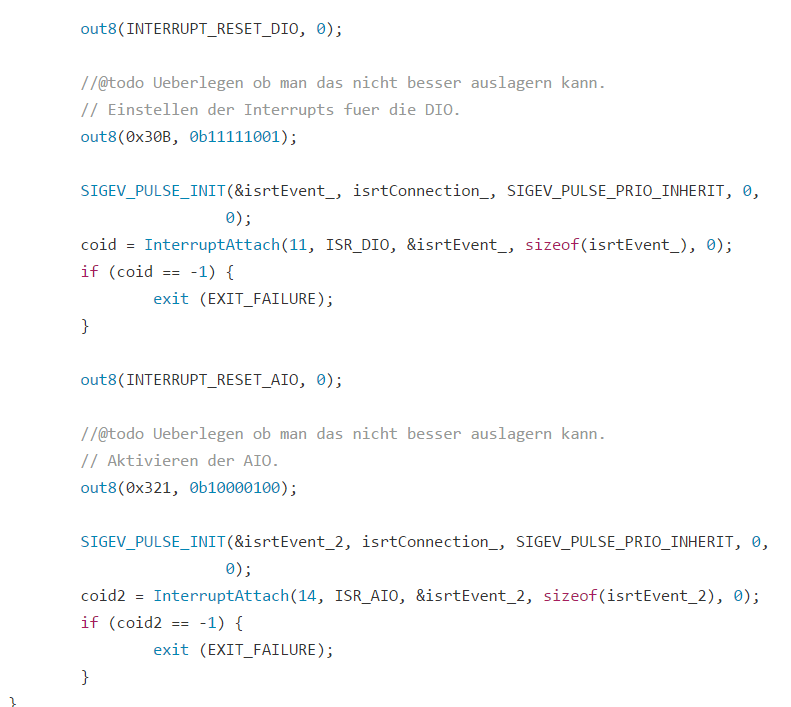
\includegraphics[scale=0.6]{ISR/regisr.png}
    
    \small Abbildung \theimgcounter : registerISR Methode aus InterruptHandler.cpp.
    \label{regisr}
\end{figure}

Die ISR von der Digitalkarte läuft so ab, dass zuerst überprüft wird, ob der Interrupt von Port B oder C kommt. Wenn dies der Fall ist, dann wird der Interrupt anschließend zurückgesetzt und der Kernel schickt eine Pulse Message mit einem Code an den SignalHandler. Der Code enthält die Information welcher Sensor den Interrupt ausgelöst hat.

\newpage

\stepcounter{imgcounter}
\begin{figure}[h]
\centering 
    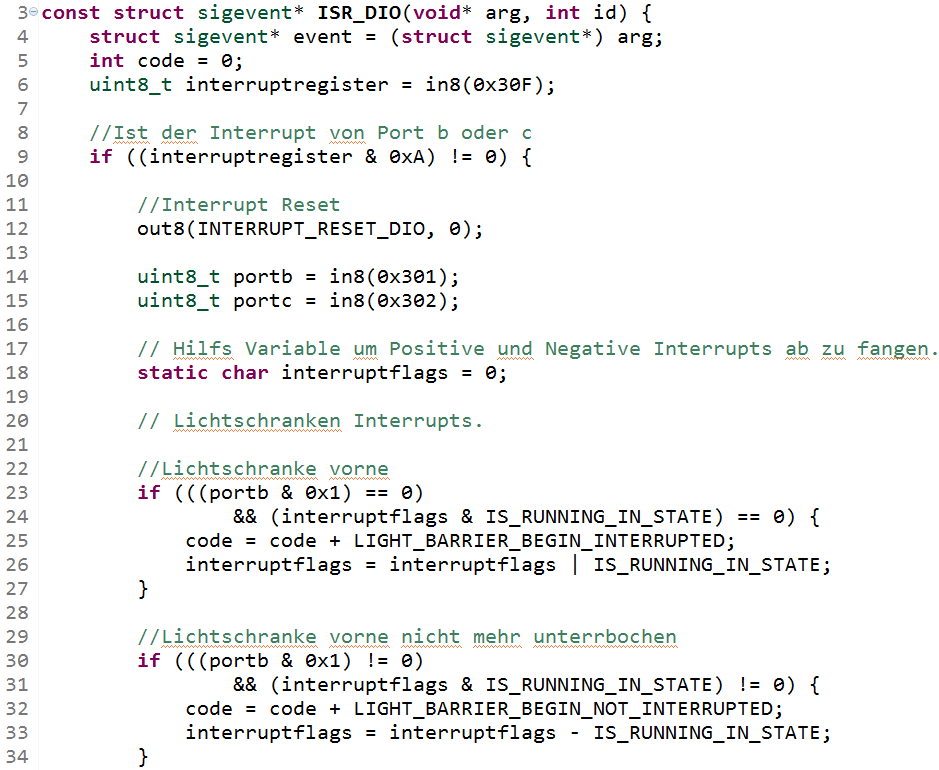
\includegraphics[scale=0.7]{ISR/isrdig.png}
    
    \small Abbildung \theimgcounter : Ausschnitt aus InterruptHandler.cpp zur Digitalkarte.
    \label{isrdig}
\end{figure}

Die ISR der Analogkarte ist für die Höhenmessung verantwortlich und läuft nach dem gleichen Prinzip wie die andere ISR ab. Es wird auch eine Pulse Message vom Kernel an den SignalHandler geschickt. Zusätzlich gibt noch eine Methode um die ISRs abzumelden.

\newpage

\subsection{Threads(SignalHandler)}
Der SignalHandlerthread empfängt alle eingehenden Pulse von der ISR(Kernel) und dem Thread von der seriellen Schnittstelle. Anschließend wird überprüft, ob ein Ereignis vorliegt und wenn ja wird es bei allen Listenern für dieses Event ausgeführt. Listener werden hinzugefügt, wenn die vordere Lichtschranke durchbrochen wird und Listener werden entfernt, wenn die Automaten den Endzustand erreicht haben. Abhängig davon welche von den drei verschiedenen Anlagen das Band ist, wird jeweils ein anderer Automat erstellt und als Listener für ein Event registriert.

\stepcounter{imgcounter}
\begin{figure}[H]
\centering
    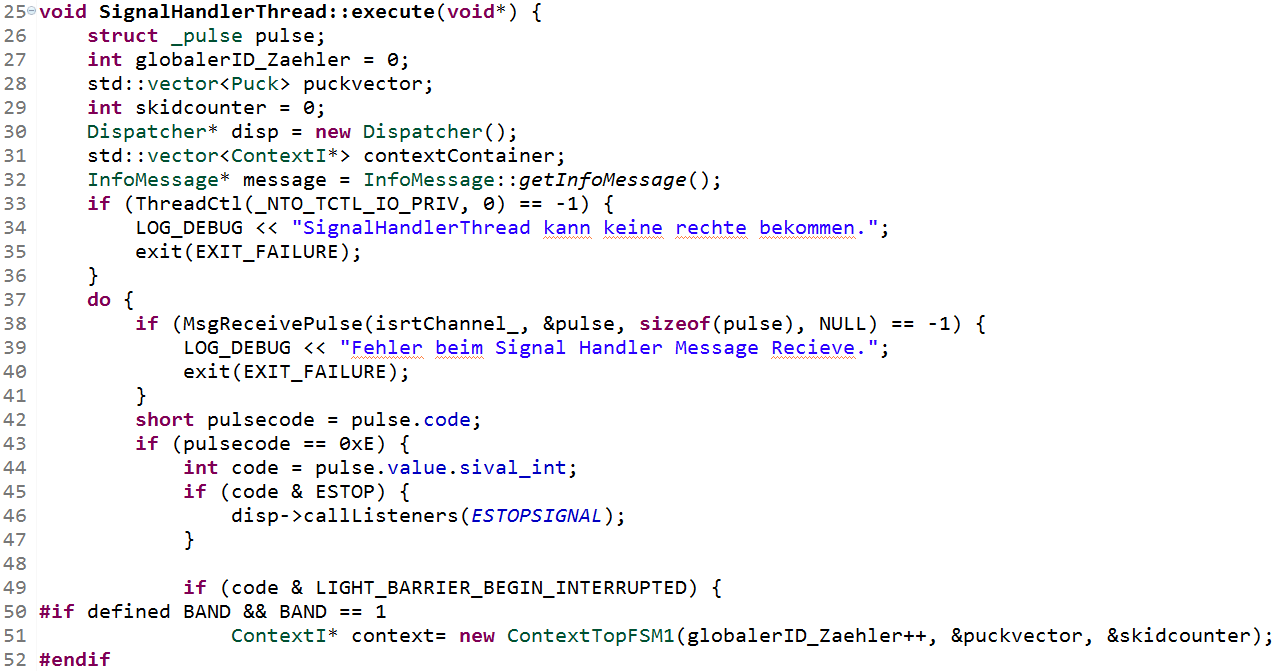
\includegraphics[scale=0.5]{ISR/sighandler.png}
    
    \small Abbildung \theimgcounter : Ausschnitt aus SignalHandlerThread.cpp. Bei Unterbrechung der vorderen Lichtschranke werden immer neue Automaten erstellt.
    \label{sighandler}
\end{figure}

\newpage

\stepcounter{imgcounter}
\begin{figure}[H]
\centering
    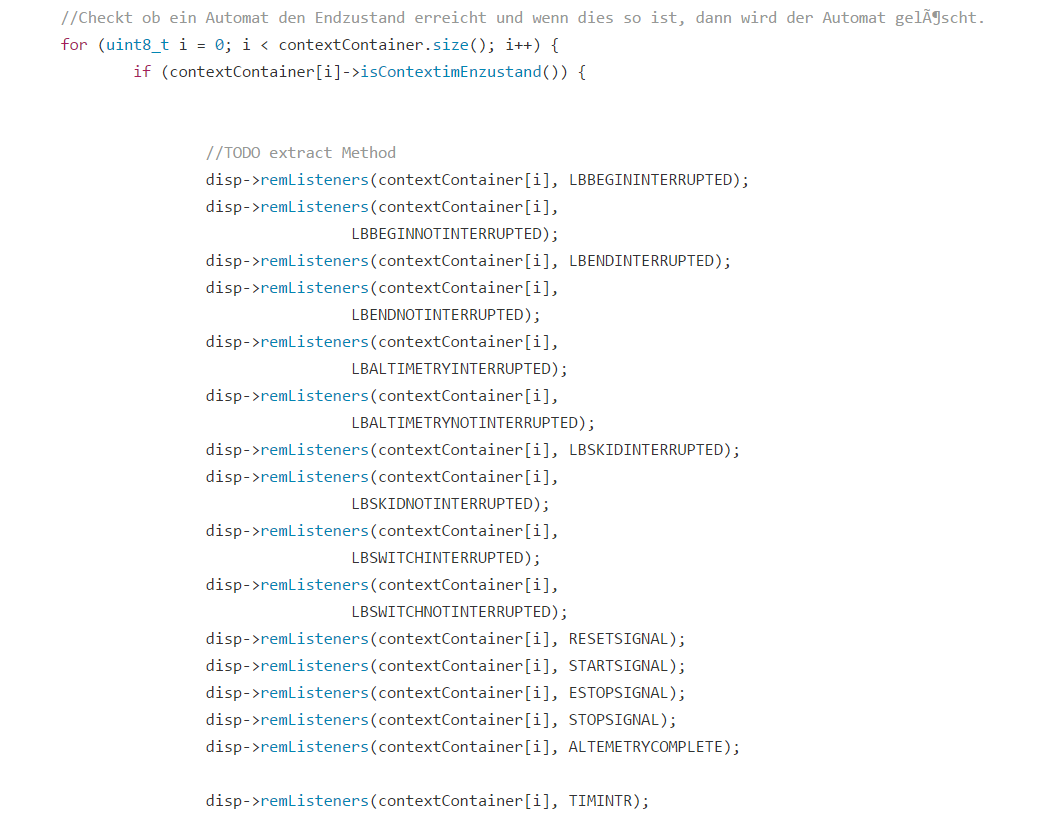
\includegraphics[scale=0.6]{ISR/dellist.png}
    
    \small Abbildung \theimgcounter : Ausschnitt aus SignalHandlerThread.cpp. Ist ein Automat im Endzustand, wird er gelöscht.
    \label{dellist}
\end{figure}

\newpage

\subsection{Dispatcher}
Der Dispatcher wendet das Observer Pattern an. Es gibt eine Methode um Listener für ein Event zu registrieren und eine Methode um Listener wieder von einem bestimmten Event abzumelden. Des Weiteren wird immer die Methode callListener aufgerufen, wenn eines der Events stattgefunden hat. Der Listener kann nun entscheiden wie und ob er auf das Event reagieren möchte. Die Listener für die Events sind Klassen(Automaten) die von einem Interface geerbt haben.

\stepcounter{imgcounter}
\begin{figure}[H]
\centering 
    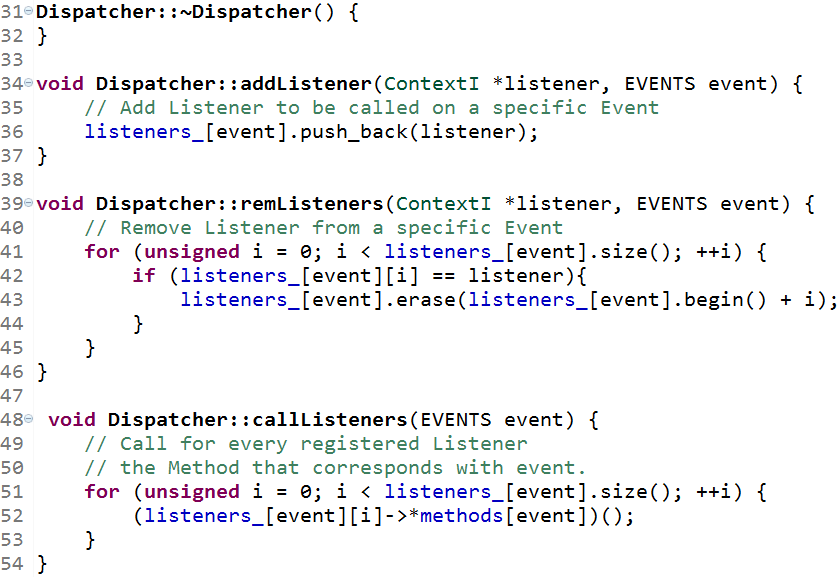
\includegraphics[scale=0.7]{ISR/dispatcher.png}
    
    \small Abbildung \theimgcounter : Die drei wichtigsten Methoden aus Dispatcher.cpp.
    \label{dispatcher}
\end{figure}

\newpage

\section{Testen}
Das Testen der Software findet nach Fertigstellung von Milestones statt, welche die Ansteuerung der Förderbänder sowie deren Kommunikation untereinander enthält. Die Tests reichen von essentiellen Ansteuerungstests einzelner Komponenten der Förderbänder bis hin zur Ablaufsteuerung über alle drei Bänder. Für die Abnahme werden definierte Tests durchgeführt.

\subsection{HAL der Aktorik}
\begin{table}[H]
\center
    \begin{tabularx}{\textwidth}{|l|X|X|X|}
        \hline
        \textbf{ID}&\textbf{Funktion}&\textbf{Test erfolgreich?}&\textbf{Anmerkung}\\
        \hline
        1&Rote Lampe an.&Ja&\\
        \hline
        2&Rote Lampe aus.&Ja&\\
        \hline
        3&Gelbe Lampe an.&Ja&\\
        \hline
        4&Gelbe Lampe aus.&Ja&\\
        \hline
        5&Grüne Lampe an.&Ja&\\
        \hline
        6&Grüne Lampe aus.&Ja&\\
        \hline
        7&Motor langsam.&Ja&\\
        \hline
        8&Motor schnell.&Ja&\\
        \hline
        9&Motor links.&Ja&\\
        \hline
        10&Motor rechts.&Ja&\\
        \hline
        11&Motor stoppen.&Ja&\\
        \hline
        12&Weiche auf.&Ja&\\
        \hline
        13&Weiche zu.&Ja&\\
        \hline
        14&Led Start an.&Ja&\\
        \hline
        15&Led Start aus.&Ja&\\
        \hline
        16&Led Reset an.&Ja&\\
        \hline
        17&Led Reset aus.&Ja&\\
        \hline
        18&Led Q1 an.&Ja&\\
        \hline
        19&Led Q1 aus.&Ja&\\
        \hline
        20&Led Q2 an.&Ja&\\
        \hline
        21&Led Q2 aus.&Ja&\\
        \hline
    \end{tabularx}
    \caption{Testauswertung zur HAL der Aktorik}
    \label{tsthal}
\end{table}

\newpage

\subsection{HAL der Sensorik}
\begin{table}[H]
\center
    \begin{tabularx}{\textwidth}{|l|X|X|X|}
        \hline
        \textbf{ID}&\textbf{Funktion}&\textbf{Test erfolgreich?}&\textbf{Anmerkung}\\
        \hline
        1&Lichtschranke Anfang unterbrochen.&Ja&\\
        \hline
        2&Lichtschranke Anfang nicht mehr unterbrochen.&Ja&\\
        \hline
        3&Lichtschranke Höhenmessung unterbrochen&Ja&\\
        \hline
        4&Lichtschranke Höhenmessung nicht mehr unterbrochen&Ja&\\
        \hline
        5&Lichtschranke Weiche unterbrochen&Ja&\\
        \hline
        6&Lichtschranke Weiche nicht mehr unterbrochen&Ja&\\
        \hline
        7&Lichtschranke Ende unterbrochen&Ja&\\
        \hline
        8&Lichtschranke Ende nicht mehr unterbrochen&Ja&\\
        \hline
        9&Lichtschranke Rutsche unterbrochen&Ja&\\
        \hline
        10&Lichtschranke Rutsche nicht mehr unterbrochen&Ja&\\
        \hline
        11&E-Stopp betätigt&Ja&\\
        \hline
        12&Stopp betätigt&Ja&\\
        \hline
        13&Start betätigt&Ja&\\
        \hline
        14&Reset betätigt&Ja&\\
        \hline
        15&Korrekte Höhenmessung&Ja&\\
        \hline
        16&Metalldetektion&Ja&\\
        \hline
    \end{tabularx}
    \caption{Testauswertung zur HAL der Sensorik}
    \label{tstsens}
\end{table}

\newpage

\subsection{Serielle Schnittstelle}
Basierend auf unseren Schnittstellen der seriellen Schnittstelle haben wir uns verschiedene Testszenarien überlegt, um die Funktionsfähigkeit und Korrektheit der Schnittstelle sicherzustellen.

\begin{table}[H]
\center
    \begin{tabularx}{\textwidth}{|l|X|l|l|}
        \hline
        \textbf{ID}&\textbf{Aktion}&\textbf{Erfolgreich?}&\textbf{Datum}\\
        \hline
        01&Kommen Nachrichten zyklisch (alle 50 ms) an der Anlage an?
        &Ja&16.12.2016\\
        \hline
        
        02&Funktionieren die Band2 Methoden:
        \begin{compactenum}[]
            \item \ttfamily InfoMessage::istBand2Frei()
            \item \ttfamily InfoMessage::setBand2Frei()
            \item \ttfamily InfoMessage::setBand2Leer()
        \end{compactenum}
        &Ja&16.12.2016\\
        \hline
        
        03&Funktionieren die Rutsche1 Methoden:
        \begin{compactenum}[] 
            \item \ttfamily InfoMessage::istBand1RutscheVoll()
            \item \ttfamily InfoMessage::setBand1RutscheVoll()
            \item \ttfamily InfoMessage::setBand1RutscheLeer()
        \end{compactenum}
        &Ja&16.12.2016\\
        \hline

        04&Funktionieren die Rutsche2 Methoden:
        \begin{compactenum}[]
            \item \ttfamily InfoMessage::istBand2RutscheVoll()
            \item \ttfamily InfoMessage::setBand2RutscheVoll()
            \item \ttfamily InfoMessage::setBand2RutscheLeer()
        \end{compactenum}
        &Ja&16.12.2016\\
        \hline
        
        05&Kommt das Ereignis SignalNextLBInterrupted an der richtigen Anlage an: 
        \begin{compactenum}[]
            \item \ttfamily InfoMessage::setLBinterruptedBit()
        \end{compactenum}
        &Ja&16.12.2016\\
        \hline
        
        06&Kommt das Ereignis EStop überall an:
        \begin{compactenum}[]
            \item \ttfamily InfoMessage::setESTOP()
            \item \ttfamily InfoMessage::removeESTOP()
        \end{compactenum}
        &Ja&16.12.2016\\
        \hline
        
        07&Funktioniert die Quittierung nicht, solange Estop gedrückt ist:
        \begin{compactenum}[]
            \item \ttfamily InfoMessage::wurdeUeberallQuitiert()
            \item \ttfamily InfoMessage::setQuittierung()
        \end{compactenum}
        &Ja&16.12.2016\\
        \hline
        
        08&Funktioniert die Quittierung:
        \begin{compactenum}[]
            \item \ttfamily InfoMessage::wurdeUeberallQuitiert()
            \item \ttfamily InfoMessage::setQuittierung()
        \end{compactenum}
        &Ja&16.12.2016\\
        \hline
        
        09&Funktioniert die Werkstückinformationsübergabe:
        {\ttfamily WorkpieceMessage::send(uint16\_t hohehnmesswert\_1, uint16\_t hohehnmesswert\_2, uint8\_t typ, uint16\_t id )}
        \begin{compactenum}[]
            \item \ttfamily struct workpiece\_package\_without\_ch 
            \item \ttfamily WorkpieceMessage::getWorkpieceInfo()
        \end{compactenum}
        &Ja&16.12.2016\\
        \hline
    \end{tabularx}
    \caption{Testauswertung zur seriellen Schnittstelle}
    \label{tstserintf}
\end{table}

\newpage

\subsection{Testszenarien}
\begin{compactenum}[1.]
    \item $\text{Flaches Werkstück} \rightarrow \text{Höhenmessung} \rightarrow$
        Band\_1 sortiert aus $\rightarrow \text{grüne Leuchte an}$
        
        [Rutsche\_1 = 1]\medskip
    \item Werkstück Bohrung unten $\rightarrow$ Höhenmessung $\rightarrow$ Band\_1 sortiert aus $\rightarrow$ grüne Leuchte an
    
        [Rutsche\_1 = 2]\medskip
    \item Werkstück Bohrung oben mit Metall $\rightarrow$ Höhenmessung $\rightarrow$ Metalldetektion $\rightarrow$ Band\_1 sortiert aus $\rightarrow$ grüne Leuchte an
    
        [Rutsche\_1 = 3]\medskip
    \item Werkstück verschwindet $\rightarrow$ Timeout $\rightarrow$ Band stoppt $\rightarrow$ gelbe Leuchte blinkt \medskip
    \item Werkstück Bohrung oben ohne Metall $\rightarrow$ Metalldetektion $\rightarrow$ Band\_1\_OK $\rightarrow$ Höhenmessung $\rightarrow$ Metalldetektion $\rightarrow$ Band\_2\_OK 
    $\rightarrow$ Band\_3\_wartet $\rightarrow$ grüne Leuchte an 
    
    [Band\_3 = 1]\medskip
    \item Werkstück Bohrung oben ohne Metall $\rightarrow$ Höhenmessung $\rightarrow$ Metalldetektion $\rightarrow$ Band\_1\_OK $\rightarrow$ Werkstück\_überschlagen $\rightarrow$ 
    Höhenmessung $\rightarrow$ Band\_2 sortiert aus $\rightarrow$ grüne Leuchte an
    
    [Rutsche\_2 = 1]\medskip
    \item Werkstück Bohrung oben mit Metall $\rightarrow$ Höhenmessung $\rightarrow$ Metalldetektion $\rightarrow$ Band\_1 sortiert aus $\rightarrow$ grüne Leuchte an
    
    [Rutsche\_1 = 4] $\rightarrow$ gelbe Leuchte an\medskip
    \item Flaches Werkstück $\rightarrow$ Band\_1\_RutscheVoll $\rightarrow$ Höhenmessung $\rightarrow$ Band\_2 sortiert aus $\rightarrow$ grüne Leuchte an
    
    [Rutsche\_2 = 2]\medskip
    \item Werkstück hinzufügen $\rightarrow$ Timeout $\rightarrow$ Band stoppt $\rightarrow$ rote Leuchte blinkt\medskip
    \item Werkstück Bohrung oben ohne Metall $\rightarrow$ Metalldetektion $\rightarrow$ Band\_1\_OK $\rightarrow$ Höhenmessung $\rightarrow$ Metalldetektion $\rightarrow$ Band\_2\_OK 
    $\rightarrow$ Band\_3\_wartet $\rightarrow$ grüne Leuchte an
    
    [Band\_3 = 2]\medskip
    \item Werkstück Bohrung unten $\rightarrow$ Band\_1\_RutscheVoll $\rightarrow$ Höhenmessung $\rightarrow$ Band\_2 sortiert aus $\rightarrow$ grüne Leuchte an
    
    [Rutsche\_2 = 3]\medskip
    \item Werkstück Bohrung oben mit Metall $\rightarrow$ Höhenmessung $\rightarrow$ Metalldetektion $\rightarrow$ Band\_1\_OK $\rightarrow$ Höhenmessung $\rightarrow$ Metalldetektion 
    $\rightarrow$ Band\_2\_OK $\rightarrow$ Band\_3\_wartet $\rightarrow$ Band\_3 Transport und Ausgabe der 3er Gruppe $\rightarrow$ grüne Leuchte an
    
    [Band\_3 = 3]\medskip
    \item Werkstück Bohrung oben ohne Metall $\rightarrow$ Höhenmessung $\rightarrow$ Metalldetektion $\rightarrow$ Band\_1\_OK $\rightarrow$ Werkstück\_überschlagen $\rightarrow$ 
    Höhenmessung $\rightarrow$ Band\_2 sortiert aus $\rightarrow$ grüne Leuchte an
    
    [Rutsche\_2 = 4]\medskip 
    \item Rutsche\_1 und Rutsche\_2 voll $\rightarrow$ Alle Förderbänder anhalten $\rightarrow$ rote Leuchte an
\end{compactenum}

\newpage

\subsection{Testkonzept für die Abnahme} 
\begin{table}[H]
\center
    \begin{tabularx}{\textwidth}{|l|X|l|l|}
        \hline
        \textbf{ID}&\textbf{Funktion}&\textbf{Erfolgreich?}&\textbf{Datum}\\
        \hline
        1&Erkennung der Werkstücke am Anfang jedes Förderbandes.&&\\
        \hline
        2&Flache Werkstücke werden auf dem ersten und zweiten Förderband aussortiert.&&\\
        \hline
        3&Werkstücke mit der Bohrung nach unten werden auf dem ersten und zweiten Förderband 
        aussortiert.&&\\
        \hline
        4&Bei voller Rutsche des ersten Förderbandes wird eine Fehlermeldung ausgegeben	und die gelbe 
        Leuchte leuchtet.&&\\
        \hline
        5&Bei voller Rutsche des zweiten Förderbandes wird eine Fehlermeldung auf der eigenen Konsole 
        ausgegeben. Das zweite Förderband stoppt und die gelbe Leuchte leuchtet.&&\\
        \hline
        6&Bei voller Rutsche vom ersten und zweiten Förderband, stoppen das erste und zweite Förderband. 
        Die rote Leuchte vom ersten und zweiten Förderband leuchtet.&&\\
        \hline
        7&Die Förderbänder stoppen jeweils, wenn sich auf ihnen keinen Werkstück befindet.&&\\
        \hline
        8&Die Förderbänder stoppen jeweils, wenn ein Werkstück auf ihnen verschwindet. Entsprechend wird 
        eine Fehlermeldung auf der eigenen Konsole ausgegeben und eigene gelbe Leuchte blinkt.&&\\
        \hline
        9&Die Förderbänder stoppen jeweils, wenn ein Werkstück mitten auf dem eigenen Laufband hinzugefügt 
        wird. Entsprechend wird eine Fehlermeldung auf der eigenen Konsole ausgegeben und die eigene rote 
        Leuchte blinkt.&&\\
        \hline
        10&Das erste Förderband sortiert die gewünschte Reihenfolge bis die eigene Rutsche voll ist.&&\\
        \hline
        11&Am Ende vom zweiten Förderband entsteht die gewünschte Reihenfolge.&&\\
        \hline
        12&Am Ende vom zweiten Förderband werden die Werkstückdaten auf der eigenen Konsole ausgegeben.&&\\
        \hline
        13&Am Ende vom dritten Förderband werden die Werkstückdaten als dreier Gruppe auf der eigenen
        Konsole ausgegeben.&&\\
        \hline
        14&Das dritte Förderband transportiert die Werkstücke erst dann bis zum Ende des Laufbandes, wenn 
        die dreier Gruppe vollständig ist.&&\\
        \hline
        15&Wenn der E-Stopp an einem der drei Förderbänder gedrückt wird, halten alle Förderbänder an.&&\\
        \hline
        16&Erst wenn alle Förderbänder nach einem Fehlerzustand quittiert wurden, kann die Anlage wieder 
        gestartet werden.&&\\
        \hline
    \end{tabularx}
    \caption{Testauswertung der Abnahmetests(Teil 1)}
    \label{tstl1}
\end{table}

\newpage

\begin{table}[H]
\center
    \begin{tabularx}{\textwidth}{|l|X|l|l|}
        \hline
        \textbf{ID}&\textbf{Funktion}&\textbf{Erfolgreich?}&\textbf{Datum}\\
        \hline

        17&Am Ende vom dritten Förderband werden die Werkstückdaten auf der Konsole als 3er Gruppe ausgegeben.&&\\
        \hline
        18&Förderband 3 transportiert die Werkstücke erst dann bis zum Ende des Bandes wenn die 3er Gruppe vollständig ist.&&\\
        \hline
        \end{tabularx}
    \caption{Testauswertung der Abnahmetests(Teil 2)}
    \label{tstl2}
\end{table}

\section{Lessons Learned}
Während des Praktikums konnten Erkenntnisse gesammelt werden, mit welcher Arbeitsweise und Planung das Team produktiv gewesen ist. Andererseits ist durch Fehlverhalten deutlich geworden, dass die Effizienz des Teams darunter leiden musste. Im Folgenden sind einige Punkte zu Pro und Contra aufgezählt, welche während eines Teammeetings zusammengetragen wurden.

\subsection{Pro}
\begin{compactenum}[$\bullet$]
\leftskip0.6cm
\item Termine eingehalten und die Zeit gut eingeteilt
\medskip
\item Durch Rollenzuweisungen konnten Kräfte optimal verteilt werden.
\medskip
\item Faire Verteilung der Aufgaben
\medskip
\item gute Planung im Voraus
\medskip
\item Konsequentes Anwenden der Visualisierungen führte zu wartbarem Code. 
\medskip
\item Gutes Teamwork
\medskip
\item Aus Fehlern gelernt
\end{compactenum}

\subsection{Contra}
\begin{compactenum}[$\bullet$]
\leftskip0.6cm
\item Zu späte Absprache über konkrete Implementierung
\medskip
\item Spätes Zusammenführen der Anlagen und Testen
\medskip
\item Späte Absprachen an den Stellen, wo zwei Teams thematisch zusammengetroffen sind (Implementation der FSMs / Dispatcher / HAL)
\end{compactenum}

\section{Anregung zum Praktikum}
Die folgenden Auflistungen zeigen Punkte auf, welche uns gut gefallen haben und welche uns negativ aufgefallen sind.

\subsection{Positiv}
\begin{compactenum}[$\bullet$]
\leftskip0.6cm
\item Tutorium war hilfreich
\medskip
\item Mangel an Kabeln wurden zügig von Enrico behoben
\medskip
\item Enrico war hilfsbereit und stets erreichbar
\medskip
\item Herr Korf war sehr hilfreich
\end{compactenum}

\subsection{Negativ}
\begin{compactenum}[$\bullet$]
\leftskip0.6cm
\item Stattfinden von Tutorium der Mechatroniker im gleichen Raum, da wir den Raum verlassen mussten und kein anderer Raum die Anlagen zu Verfügung stellt.
\medskip
\item Räume zu voll daher keine Anlagen frei gewesen
\medskip
\item Bei drei Anlagen war es immer schwer alle Förderbänder und Kabel parat zu haben, weshalb die Planung verändert/verzögert werden musste.
\end{compactenum}

\end{document}

% Weitere Syntax für verschiedene Anwendungsfelder

%Aufzählungen
%\begin{compactenum}[1.]
%\item
%\end{compactenum}

%\ref{labelname des zu Referenzierenden Objekts}

%Tabelle
%\begin{table}[h]
%\center
%\begin{tabular}{|l|l|}
%\hline
%\textbf{linke Spaltenüberschrift}&\textbf{rechte Spaltenüberschrift}\\
%\hline
%1&2\\
%\hline
%3&4\\
%\end{tabular}
%\caption{Zugriffsoperationen}
%\label{labelname}
%\end{table}

%Tabelle mit tabularx
%\begin{table}[h]
%\center
%\begin{tabularx}{\textwidth}{|l|X|}
%\hline
%Text in linker Spalte&Text in rechter Spalte der über den Rand hinausragt\\
%\hline
%\end{tabularx}
%\caption{Tabellenunterschrift}
%\label{labelname}
%\end{table}

%Grafik einfügen
%\begin{figure}[h]
%\centering 
%\includegraphics[scale=0.3]{Dateiname}
%\caption{Bildunterschrift}
%\label{labelname}
%\end{figure}

%Linksbündig mit definierter Einrückung
%\begin{flushleft}
%\leftskip0.6cm
%\end{flushleft}

%Codelisting
%\lstset{basicstyle=\ttfamily}
%\begin{lstlisting}
%Code
%\end{lstlisting}

%Erzeugen eines Inhaltsverzeichnisses und ihrer Einträge
%\tableofcontents
%\section{•}
%\subsection{•}

%Vertikaler Abstand
%\vspace{0cm}

%Etwas zentrieren
%\centering 

%Um PDFs skaliert einzufügen und Seitenzahl sowie header beizubehalten 
%\includepdf[pages={2}, nup=1x1, scale=0.9, pagecommand={}]{file.pdf}

%Um PDFs ohne Skalierung einzufügen und Seitenzahl sowie header beizubehalten 
%\label{labelname}\hypertarget{haluml}{}
%\includepdf[pages=1,pagecommand={}]{file.pdf}

%Um PDFs einfach einzufügen, Seitenzahl, header und footer werden überlagert
%\includepdf[landscape=true,pages=-]{file.pdf}

%Um PDFs mit vorangehendem Text einzufügen mit Skalierung
%\includepdf[scale=0.8,pages=1,pagecommand=\subsection{Kapitel} Text]{file.pdf}

%Literaturverzeichnis anlegen
%\bibliography{Literaturverzeichnis}